\chapter{Neural Networks}

Humans have always considered themselves intelligent, perhaps too intelligent. For centuries, philosophers, anatomists, and scientists stared into the mirror of the mind, trying to grasp what makes intelligence possible. Naturally, the question arose: \textit{How do we think?} And if we could understand that, \textit{could we build a machine that thinks?} To build an artificial intelligence, we need to take inspiration from nature's most optimized real intelligent machine — the brain!

\section{The Neuron}

In 1873, an Italian scientist named \textit{\textbf{Camillo Golgi}} discovered a silver staining technique that revealed something extraordinary: the fine cellular architecture of the brain. In 1890, a Spanish neuroscientist and artist, \textit{\textbf{Santiago Ramón y Cajal}} took Golgi's stain and produced breathtaking drawings that showed brain as connected architecture of individual, separate units --- not a continuous mesh as many thought. Cajal proposed what we now call the \textit{Neuron Doctrine}: that the brain is made up of individual units, now known as \textbf{neurons}, that communicate across small gaps by transmitting chemicals (signals), which we now call \textbf{synapses}. 

The exact working of the brain was little understood by the 1940s. However, one thing was known: neurons form a network, and based on the signals they receive from other neurons, they decide whether to release a signal themselves, a process called \textit{firing}, or not. Enter \textit{\textbf{Warren McCulloch}}, a neurophysiologist, and \textit{\textbf{Walter Pitts}}, a brilliant young logician who had taught himself formal logic as a teenager. In 1943, in a small research lab in Chicago, they published a revolutionary paper: \textit{A Logical Calculus of the Ideas Immanent in Nervous Activity} \cite{mcculloch_pitts}. 

In their paper they proposed that each neuron functions as a binary threshold unit. Neurons receive multiple input signals, aggregate them, and produce an output (i.e., \textit{fire}) only if the aggregated signal crosses a certain threshold. Formally, the \textbf{McCulloch-Pitts model} defines a neuron that receives inputs $\mathbf{x} = (x_1,\text{ }x_2,\text{ } \dots, \text{ }x_n)$, where any input $x_i \in \{0, 1\}$. The neuron aggregates the inputs by computing the sum $g(\mathbf{x}) = \sum_{i=1}^{n} x_i$. 

The output is then determined by a fixed constant known as the \textit{thresholding parameter}, $\theta$, as
$$
y = f(g(\mathbf{x})) = 
\begin{cases}
1 & \text{if } g(\mathbf{x}) \geq \theta \\
0 & \text{if } g(\mathbf{x}) < \theta
\end{cases}
$$

Geometrically, a single McCulloch-Pitts neuron divides the space of input points into two regions by a decision boundary defined by the equation $\sum_{i=1}^n x_i - \theta = 0$. For the case of two binary inputs, this line partitions the four possible input points into two groups: those for which $\sum x_i < \theta$ (which produce output 0) and those for which $\sum x_i \geq \theta$ (which produce output 1). Thus, the decision boundary acts as a separator in the input space.

This idea naturally extends to higher dimensions. If the neuron receives three inputs, the line becomes a plane: $\sum_{i=1}^3 x_i - \theta = 0$. For instance, in the case of the 3-input OR function, the desired plane must separate the point (0,0,0) which should produce output 0, from the other seven binary combinations, which should all produce output 1.

\begin{figure}[h]
    \centering
    \subfloat[AND Gate]{
        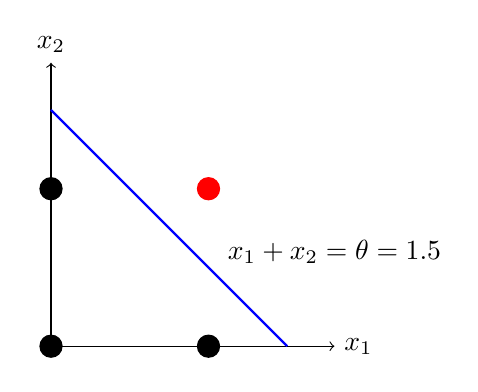
\begin{tikzpicture}[scale=2]
            \draw[->] (0,0) -- (1.8,0) node[right] {$x_1$};
            \draw[->] (0,0) -- (0,1.8) node[above] {$x_2$};

            \filldraw[black] (0,0) circle (2pt);
            \filldraw[black] (1,0) circle (2pt);
            \filldraw[black] (0,1) circle (2pt);
            \filldraw[red] (1,1) circle (2pt);

            \draw[thick, blue] (0,1.5) -- (1.5,0);
            \node at (1.8,0.6) [black] {$x_1 + x_2 = \theta = 1.5$};
        \end{tikzpicture}
    }
    \hspace{80pt}
    \subfloat[OR Gate]{
        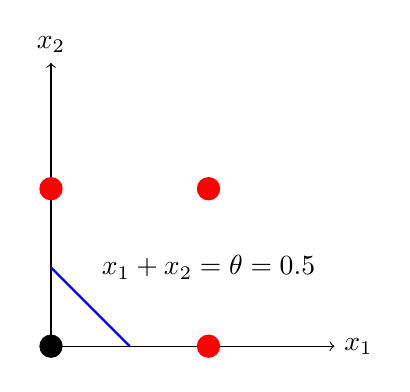
\begin{tikzpicture}[scale=2]
            \draw[->] (0,0) -- (1.8,0) node[right] {$x_1$};
            \draw[->] (0,0) -- (0,1.8) node[above] {$x_2$};

            \filldraw[black] (0,0) circle (2pt);
            \filldraw[red] (1,0) circle (2pt);
            \filldraw[red] (0,1) circle (2pt);
            \filldraw[red] (1,1) circle (2pt);

            \draw[thick, blue] (0,0.5) -- (0.5,0);
            \node at (1,0.5) [black] {$x_1 + x_2 = \theta = 0.5$};
        \end{tikzpicture}
    }
    \caption{McCulloch-Pitts neuron implementing logical functions via thresholding}
\end{figure}

The McCulloch-Pitts neuron provides a foundational abstraction of a biological neuron, but it also raises several important questions. \textit{What if the inputs are not binary but real-valued? Do we always need to manually specify the threshold parameter? Are all inputs equally important, or should some be assigned more weight?} Finally, \textit{can such a neuron model functions that are not linearly separable?}


\section{The Perceptron}

To address these concerns, \textit{\textbf{Frank Rosenblatt}} introduced the \textit{Perceptron} in 1958, funded by the U.S. Navy. Rosenblatt's model generalized the McCulloch-Pitts neuron by allowing real-valued inputs, learnable weights, and thresholds.

Formally, the perceptron computes a weighted sum of its inputs and applies a threshold to determine the binary output.
\[
y =
\begin{cases}
1 & \text{if } \sum_{i=1}^{n} w_i x_i - \theta \geq 0 \\
0 & \text{if } \sum_{i=1}^{n} w_i x_i - \theta < 0
\end{cases}
\]

A more commonly used convention rewrites this using a \textit{bias} term.
\[
y =
\begin{cases}
1 & \text{if } \sum_{i=0}^{n} w_i x_i \geq 0 \\
0 & \text{if } \sum_{i=0}^{n} w_i x_i < 0
\end{cases}
\quad \text{where } x_0 = 1 \text{ and } w_0 = -\theta
\]

This formulation shows that a perceptron still divides the input space into two halves. Inputs that produce an output of 1 lie on one side of the decision boundary $\sum w_i x_i = 0$, while those producing 0 lie on the other. 

In other words, a single perceptron can only model linearly separable functions. However, it differs from the McCulloch-Pitts model in two significant ways: the weights (including the threshold) are learnable from data, and the inputs can be real-valued.

Let us revisit the Boolean OR function. For inputs $x_1, x_2 \in \{0,1\}$, we desire an output $y = x_1 \lor x_2$. The perceptron should satisfy the following inequalities. 

\begin{table}[h]
\centering
\begin{tabular}{ccccl}
$\mathbf{x_1}$ & $\mathbf{x_2}$ & \textbf{OR} & \textbf{Inequality} & \textbf{Condition} \\
\hline
0 & 0 & 0 & $w_0 + w_1 \cdot 0 + w_2 \cdot 0 < 0$ & $\Rightarrow w_0 < 0$ \\
1 & 0 & 1 & $w_0 + w_1 \cdot 1 + w_2 \cdot 0 \geq 0$ & $\Rightarrow w_1 \geq -w_0$ \\
0 & 1 & 1 & $w_0 + w_1 \cdot 0 + w_2 \cdot 1 \geq 0$ & $\Rightarrow w_2 \geq -w_0$ \\
1 & 1 & 1 & $w_0 + w_1 \cdot 1 + w_2 \cdot 1 \geq 0$ & $\Rightarrow w_1 + w_2 \geq -w_0$
\end{tabular}
\caption{Linear inequalities that represent the OR gate using weights $w_0$, $w_1$, and $w_2$}
\end{table}


One possible solution satisfying all the above constraints is
\(
w_0 = -1, \text{ } w_1 = 1.1, \text{ and } w_2 = 1.1. 
\)

Note that this is not a unique solution—many combinations of weights satisfy the inequalities. The key insight is that for linearly separable functions like OR, a perceptron can find suitable weights to model the function accurately. We will later explore how these weights can be learned automatically using the \textit{perceptron learning algorithm} \cite{khapra2018deeplearning}.

\subsection{Perceptron Learning Algorithm}

Imagine we want to make a binary decision of whether to watch a movie or not. Suppose we are given a list of $m$ movies, each labeled as either liked (1) or not liked (0) by a user. Each movie is represented by $n$ features, which can be either Boolean or real-valued. We assume the data is linearly separable and aim to train a perceptron to learn this classification rule. In other words, we want the perceptron to find the parameters $\mathbf{w} = [w_0, w_1, \ldots, w_n]$ that define a separating hyperplane.

We now describe the perceptron learning algorithm formally.

\begin{algobox}{Perceptron Learning Algorithm}
Let $P \gets$ set of inputs labeled $1$ \\
 Let $N \gets$ set of inputs labeled $0$ \\
 Initialize weight vector $\mathbf{w}$ randomly \\
 \textbf{while} not converged \textbf{do} \\
\hspace*{1em}  Pick a random example $\mathbf{x} \in P \cup N$ \\
\hspace*{1em}  \textbf{if} $\mathbf{x} \in P$ and $\mathbf{w}^T \mathbf{x} < 0$ \textbf{then} \\
\hspace*{2em}  $\mathbf{w} \gets \mathbf{w} + \mathbf{x}$ \\
\hspace*{1em}  \textbf{if} $\mathbf{x} \in N$ and $\mathbf{w}^T \mathbf{x} \geq 0$ \textbf{then} \\
\hspace*{2em}  $\mathbf{w} \gets \mathbf{w} - \mathbf{x}$ \\
 \textbf{end while}
\end{algobox}

The algorithm continues updating the weights until all inputs are correctly classified. \textit{But why does this work?}

To understand this, consider two vectors: the weight vector $\mathbf{w} = [w_0, w_1, \ldots, w_n]$ and an input vector $\mathbf{x} = [1, x_1, \ldots, x_n]$. The perceptron computes the dot product 
\[
\mathbf{w} \cdot \mathbf{x} = \mathbf{w}^T \mathbf{x} = \sum_{i=0}^{n} w_i x_i
\]
The classification rule can then be written as 
\[
y =
\begin{cases}
1 & \text{if } \mathbf{w}^T \mathbf{x} \geq 0 \\
0 & \text{if } \mathbf{w}^T \mathbf{x} < 0
\end{cases}
\]

Geometrically, the equation $\mathbf{w}^T \mathbf{x} = 0$ defines a hyperplane that splits the input space into two halves. Any point $\mathbf{x}$ lying on this hyperplane satisfies $\mathbf{w}^T \mathbf{x} = 0$. The weight vector $\mathbf{w}$ is orthogonal to this hyperplane, because the angle $\alpha$ between $\mathbf{w}$ and any vector $\mathbf{x}$ on the hyperplane is $90^\circ$, which implies $\cos \alpha = 0$ and hence $\mathbf{w}^T \mathbf{x} = 0$.

Now consider a point $\mathbf{x} \in P$ (positive class) such that $\mathbf{w}^T \mathbf{x} < 0$. This implies that the angle between $\mathbf{w}$ and $\mathbf{x}$ is greater than $90^\circ$, i.e., $\mathbf{x}$ lies in the wrong half-space. We wish to reduce this angle so that $\mathbf{x}$ lies in the correct half-space. Updating $\mathbf{w} \gets \mathbf{w} + \mathbf{x}$ has the following effect
\[
\mathbf{w}_{\text{new}}^T \mathbf{x} = (\mathbf{w} + \mathbf{x})^T \mathbf{x} = \mathbf{w}^T \mathbf{x} + \mathbf{x}^T \mathbf{x}
\]
Since $\mathbf{x}^T \mathbf{x} > 0$, we have $\mathbf{w}_{\text{new}}^T \mathbf{x} > \mathbf{w}^T \mathbf{x}$, which implies $\cos(\alpha_{\text{new}}) > \cos(\alpha)$ and therefore $\alpha_{\text{new}} < \alpha$. This update moves the decision boundary in the desired direction, reducing misclassification.

Similarly, for a point $\mathbf{x} \in N$ (negative class) such that $\mathbf{w}^T \mathbf{x} \geq 0$, the vector $\mathbf{x}$ lies in the wrong half-space. The angle between $\mathbf{w}$ and $\mathbf{x}$ is less than $90^\circ$. Updating $\mathbf{w} \gets \mathbf{w} - \mathbf{x}$ yields
\[
\mathbf{w}_{\text{new}}^T \mathbf{x} = (\mathbf{w} - \mathbf{x})^T \mathbf{x} = \mathbf{w}^T \mathbf{x} - \mathbf{x}^T \mathbf{x}
\]
Since $\mathbf{x}^T \mathbf{x} > 0$, this results in $\mathbf{w}_{\text{new}}^T \mathbf{x} < \mathbf{w}^T \mathbf{x}$, i.e., $\cos(\alpha_{\text{new}}) < \cos(\alpha)$ and thus $\alpha_{\text{new}} > \alpha$. The update moves the vector $\mathbf{w}$ further from $\mathbf{x}$, pushing the decision boundary away from misclassified negative points.

This geometric intuition explains why the perceptron algorithm always converges for linearly separable data. At each step, it reduces the number of misclassified points by rotating the decision boundary in the correct direction.

\begin{definition}
Two sets $P$ and $N$ of points in an $n$-dimensional space are called \textit{absolutely linearly separable} if there exist $n + 1$ real numbers $w_0, w_1, \ldots, w_n$ such that every point $(x_1, x_2, \ldots, x_n) \in P$ satisfies $\sum_{i=1}^n w_i x_i > w_0$ and every point $(x_1, x_2, \ldots, x_n) \in N$ satisfies $\sum_{i=1}^n w_i x_i < w_0$.
\end{definition}

\begin{theorem}
If the sets $P$ and $N$ are finite and linearly separable, the perceptron learning algorithm updates the weight vector $\mathbf{w}_t$ only a finite number of times. In other words, if the vectors in $P$ and $N$ are tested cyclically, a weight vector $\mathbf{w}_t$ is found after a finite number of steps $t$ which separates the two sets.
\end{theorem}

\textit{Proof.} If $\mathbf{x} \in N$, then $-\mathbf{x} \in P'$, where $P' = P \cup \{-\mathbf{x} : \mathbf{x} \in N\}$. This is because if $\mathbf{w}^T \mathbf{x} < 0$, then $\mathbf{w}^T (-\mathbf{x}) > 0$.

Hence, we can consider a unified set $P'$ where every element $\mathbf{p} \in P'$ satisfies $\mathbf{w}^T \mathbf{p} \geq 0$. Without loss of generality, normalize all vectors $\mathbf{p}$ so that $\|\mathbf{p}\| = 1$. This normalization does not affect the separating condition since $\mathbf{w}^T \mathbf{p}/\|\mathbf{p}\| \geq 0$ implies $\mathbf{w}^T \mathbf{p} \geq 0$.

Let $\mathbf{w}^*$ be the normalized ideal weight vector such that $\mathbf{w}^{*T} \mathbf{p} > 0$ for all $\mathbf{p} \in P'$. Define $\delta = \min_{\mathbf{p} \in P'} \mathbf{w}^{*T} \mathbf{p} > 0$.

Now, suppose at time $t$ we inspect point $\mathbf{p}_i \in P'$ and find $\mathbf{w}_t^T \mathbf{p}_i \leq 0$. A correction is made: \[ \mathbf{w}_{t+1} = \mathbf{w}_t + \mathbf{p}_i. \]

Let $\beta$ be the angle between $\mathbf{w}_{t+1}$ and $\mathbf{w}^*$. Then,
\[
\cos \beta = \frac{\mathbf{w}^* \cdot \mathbf{w}_{t+1}}{\|\mathbf{w}_{t+1}\|} = \frac{\mathbf{w}^* \cdot (\mathbf{w}_t + \mathbf{p}_i)}{\|\mathbf{w}_{t+1}\|} = \frac{\mathbf{w}^* \cdot \mathbf{w}_t + \mathbf{w}^* \cdot \mathbf{p}_i}{\|\mathbf{w}_{t+1}\|}.
\]
Since $\mathbf{w}^* \cdot \mathbf{p}_i \geq \delta$, we obtain
\[ \mathbf{w}^* \cdot \mathbf{w}_{t+1} \geq \mathbf{w}^* \cdot \mathbf{w}_t + \delta. \]
By induction, after $k$ corrections, we have
\[ \mathbf{w}^* \cdot \mathbf{w}_t \geq \mathbf{w}^* \cdot \mathbf{w}_0 + k\delta. \]

Now consider the squared norm of $\mathbf{w}_{t+1}$:
\[
\|\mathbf{w}_{t+1}\|^2 = \|\mathbf{w}_t + \mathbf{p}_i\|^2 = \|\mathbf{w}_t\|^2 + 2 \mathbf{w}_t \cdot \mathbf{p}_i + \|\mathbf{p}_i\|^2.
\]
Since $\mathbf{w}_t \cdot \mathbf{p}_i \leq 0$ and $\|\mathbf{p}_i\| = 1$, we get
\[ \|\mathbf{w}_{t+1}\|^2 \leq \|\mathbf{w}_t\|^2 + 1. \]
Inductively,
\[ \|\mathbf{w}_t\|^2 \leq \|\mathbf{w}_0\|^2 + k. \]

Putting everything together,
\[
\cos \beta = \frac{\mathbf{w}^* \cdot \mathbf{w}_t}{\|\mathbf{w}_t\|} \geq \frac{\mathbf{w}^* \cdot \mathbf{w}_0 + k\delta}{\sqrt{\|\mathbf{w}_0\|^2 + k}}.
\]

As $k$ increases, the numerator grows linearly, but the denominator grows as $\sqrt{k}$, so $\cos \beta$ can grow unbounded. However, since $\cos \beta \leq 1$, the number of corrections $k$ must be bounded. Therefore, the perceptron algorithm must converge after a finite number of updates.

Let's have a look back at the questions raised after McCulloch-Pitts model. 

\textit{What if the inputs are not binary but real-valued?}
The perceptron works directly with real-valued inputs, using the sign of the weighted sum $\mathbf{w}^\top \mathbf{x}$ to make decisions.

\textit{Do we always need to manually specify the threshold parameter?}
No, the threshold can be learned as a bias term $w_0$ by appending a constant $x_0 = 1$ to the input vector.

\textit{Are all inputs equally important, or should some be assigned more weight?}
Inputs can have different importance, reflected in the learned weights $\mathbf{w}$, which adjust based on the training data.

\textit{Can such a neuron model functions that are not linearly separable?}
No, a single perceptron can only separate linearly separable data. We will see soon how to handle this. 

This section was developed in 1969 by two prominent MIT scientists, \textit{\textbf{Marvin Minsky}} and \textit{\textbf{Seymour Papert}}. In their book, \textit{Perceptrons}, they critically analyzed the limitations of Rosenblatt's model. They mathematically proved the above mentioned \textit{perceptron learning algorithm} and showed that a single perceptron could not solve non-linearly separable problems, such as the simple XOR function.

Their critique wasn't wrong but the fallout was dramatic. Funding dried up. Neural networks were declared a dead end. For nearly a decade, research interest in neural models collapsed.

\subsection{Layer of Perceptrons}

\textit{How many boolean functions can you design from $n$ inputs?} $2^{2^n}$. Some of them are not linear separable. There is no general formula that tells us that. For 2 input example, there are 16 possible boolean functions, of which XOR and !XOR are not linearly separable. 

\begin{table}[h]
\centering
\begin{tabular}{cc|cccccccccccccccc}
$x_1$ & $x_2$ & $f_1$ & $f_2$ & $f_3$ & $f_4$ & $f_5$ & $f_6$ & $f_7$ & $f_8$ & $f_9$ & $f_{10}$ & $f_{11}$ & $f_{12}$ & $f_{13}$ & $f_{14}$ & $f_{15}$ & $f_{16}$ \\
\hline
0 & 0 & 0 & 0 & 0 & 0 & 0 & 0 & 0 & 0 & 1 & 1 & 1 & 1 & 1 & 1 & 1 & 1 \\
0 & 1 & 0 & 0 & 0 & 0 & 1 & 1 & 1 & 1 & 0 & 0 & 0 & 0 & 1 & 1 & 1 & 1 \\
1 & 0 & 0 & 0 & 1 & 1 & 0 & 0 & 1 & 1 & 0 & 0 & 1 & 1 & 0 & 0 & 1 & 1 \\
1 & 1 & 0 & 1 & 0 & 1 & 0 & 1 & 0 & 1 & 0 & 1 & 0 & 1 & 0 & 1 & 0 & 1 \\
\end{tabular}
\caption{Functions $f_1$ to $f_{16}$ for input combinations of $x_1$ and $x_2$}
\end{table}

\begin{figure}[h!]
\centering
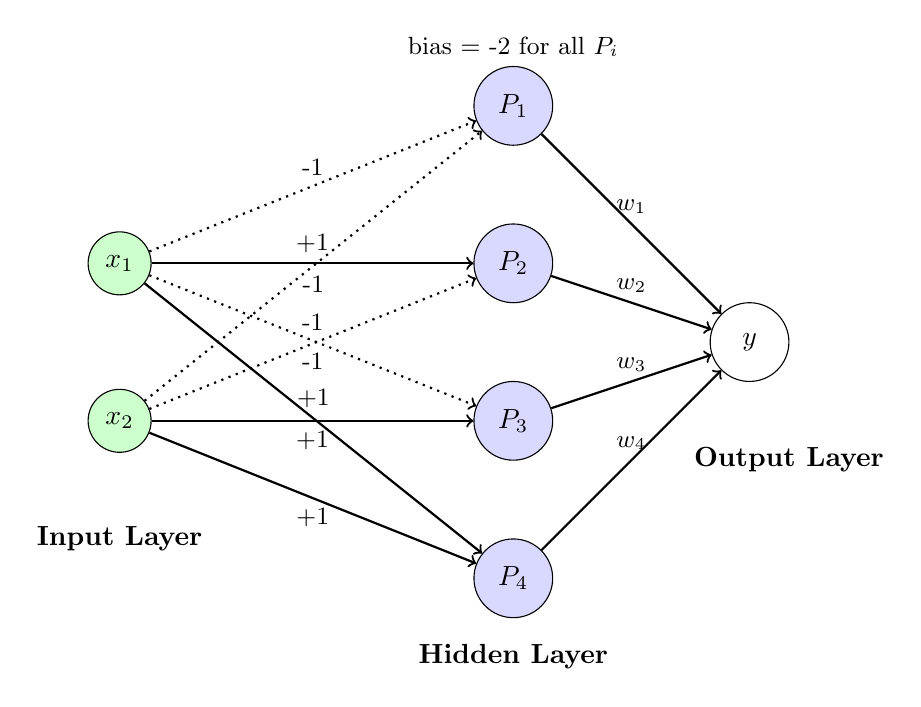
\begin{tikzpicture}[
    neuron/.style={circle, draw, minimum size=1cm, fill=blue!15},
    input/.style={circle, draw, minimum size=0.8cm, fill=green!20},
    output/.style={circle, draw, minimum size=1cm},
    weight/.style={font=\small, midway, above},
    bias/.style={font=\small, below},
    arrow/.style={->, thick},
    positive/.style={->, thick},
    negative/.style={->, thick, dotted}
]

% Input layer
\node[input] (x1) at (0, 2) {$x_1$};
\node[input] (x2) at (0, 0) {$x_2$};

% Hidden layer (4 perceptrons)
\node[neuron] (p1) at (5, 4) {$P_1$};
\node[neuron] (p2) at (5, 2) {$P_2$};
\node[neuron] (p3) at (5, 0) {$P_3$};
\node[neuron] (p4) at (5, -2) {$P_4$};

% Output layer
\node[output] (y) at (8, 1) {$y$};

% Input to hidden layer connections
\draw[negative] (x1) -- (p1) node[weight] {-1};
\draw[negative] (x2) -- (p1) node[weight, below] {-1};

\draw[positive] (x1) -- (p2) node[weight] {+1};
\draw[negative] (x2) -- (p2) node[weight, below] {-1};

\draw[negative] (x1) -- (p3) node[weight] {-1};
\draw[positive] (x2) -- (p3) node[weight, below] {+1};

\draw[positive] (x1) -- (p4) node[weight] {+1};
\draw[positive] (x2) -- (p4) node[weight, below] {+1};

% Hidden to output layer connections
\draw[arrow] (p1) -- (y) node[weight] {$w_1$};
\draw[arrow] (p2) -- (y) node[weight] {$w_2$};
\draw[arrow] (p3) -- (y) node[weight] {$w_3$};
\draw[arrow] (p4) -- (y) node[weight] {$w_4$};

% Bias annotations
\node[bias] at (5, 5) {bias = -2 for all $P_i$};

% Labels
\node at (0, -1.5) {\textbf{Input Layer}};
\node at (5, -3) {\textbf{Hidden Layer}};
\node at (8.5, -0.5) {\textbf{Output Layer}};

\end{tikzpicture}
\caption{Two Input Network with Four Hidden Perceptrons}
\end{figure}

Two binary inputs, $x_1$ and $x_2$, are passed to a hidden layer with four perceptrons $P_1$ to $P_4$. Each perceptron in the hidden layer computes a distinct linear combination of the inputs with weights $\pm1$, effectively separating different input regions. All hidden units use a fixed bias of $-2$. The outputs from the hidden layer are linearly combined in the output layer using learnable weights $w_1, w_2, w_3, w_4$ to produce the final output $y$. 

This network can implement \textit{any boolean function}, whether linearly separable or not. The key idea lies in the design of the hidden layer. Each of the four perceptrons is constructed to \textit{fire (output 1) for exactly one of the four possible input combinations} of $(x_1, x_2)$, and \textit{only} for that combination.

\begin{table}[h]
\centering
\begin{tabular}{cc}
\textbf{Perceptron} & \textbf{Input that Activates It} \\
\hline
$P_1$ & $(0, 0)$ \\
$P_2$ & $(0, 1)$ \\
$P_3$ & $(1, 0)$ \\
$P_4$ & $(1, 1)$ \\
\end{tabular}
\caption{Unique input activation for each perceptron}
\end{table}

Because each hidden unit uniquely represents one input, the output neuron can now learn the desired boolean function by \textit{assigning appropriate weights} $w_1, w_2, w_3, w_4$ to these hidden activations. For instance, to implement XOR, we can simply set the weights such that the output neuron fires for $(0,1)$ and $(1,0)$, and stays off for $(0,0)$ and $(1,1)$. This translates to the following conditions.
\[
w_1 < w_0,\quad w_2 \geq w_0,\quad w_3 \geq w_0,\quad w_4 < w_0
\]
There are \textit{no contradictions}. Thus, by adjusting the output weights accordingly, this single network architecture can represent \textit{all 16 possible boolean functions}.

\begin{theorem}
    Any boolean function of \( n \) inputs can be represented exactly by a network of perceptrons containing one hidden layer with \( 2^n \) perceptrons and one output layer containing a single perceptron \cite{khapra2018deeplearning}.
\end{theorem}

\begin{proof}
A boolean function \( f: \{0,1\}^n \to \{0,1\} \) is defined on \( 2^n \) possible input vectors.

Construct a hidden layer with \( 2^n \) perceptrons, each configured to activate only for one unique input vector by appropriate weights and bias.

The output perceptron then sums the hidden layer outputs with weights chosen to output 1 exactly for inputs where \( f \) is 1, and 0 otherwise.

Thus, the network exactly represents any boolean function.
\end{proof}

\begin{quote}
    \textbf{Note:} A network with \( 2^n + 1 \) perceptrons is not necessary but sufficient. For example, we have seen how to represent the OR function (and similarly AND function)    with just one perceptron.
\end{quote}

\begin{quote}
    \textbf{Catch:} As \( n \) increases, the number of perceptrons in the hidden layer increases exponentially.
\end{quote}
\section{The Sigmoid Neuron}

The perceptron's thresholding logic is quite harsh. Consider a simple example where we decide whether to like or dislike a movie based on a single input: \textit{the critic's rating} \( x_1 \), which ranges from 0 to 1. Suppose the threshold is set at 0.5, with weights \( w_0 = -0.5 \) and \( w_1 = 1 \). For a movie with \( x_1 = 0.51 \), the perceptron outputs \textit{like,} while for \( x_1 = 0.49 \), it outputs \textit{dislike.} This sudden change in decision seems strict and abrupt.

This behavior is not due to the specific problem or chosen weights. Instead, it is inherent to the perceptron function, which acts as a step function. The output switches sharply from 0 to 1 when the weighted sum
\(
\sum_{i=1}^n w_i x_i
\)
crosses the threshold \(-w_0\).

In real-world cases, we usually want a smoother decision function that changes gradually from 0 to 1. This motivates the introduction of sigmoid neurons, where the output function is continuous and smooth.

One common sigmoid function is the logistic function, defined as
\[
y = \frac{1}{1 + e^{-(w_0 + \sum_{i=1}^n w_i x_i)}}
\]
Here, the output \( y \) does not jump suddenly but transitions smoothly around the threshold \(-w_0\).

Moreover, the output \( y \) is no longer binary; it takes values between 0 and 1. This output can be interpreted as a probability. So instead of a hard like/dislike decision, we get the probability of liking the movie.

\begin{figure}[ht]
    \centering
    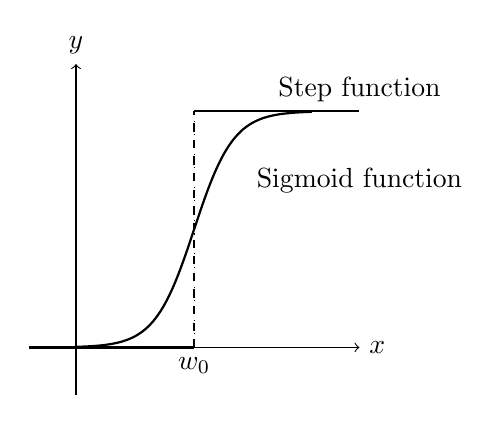
\begin{tikzpicture}[scale=3]
        % Axes
        \draw[->] (-0.2,0) -- (1.2,0) node[right] {$x$};
        \draw[->] (0,-0.2) -- (0,1.2) node[above] {$y$};

        % Step function (Perceptron)
        \draw[thick] (-0.2,0) -- (0.5,0);
        \draw[thick] (0.5,1) -- (1.2,1);
        \draw[thick,dashed] (0.5,0) -- (0.5,1);
        \node[above] at (1.2,1) {Step function};

        % Sigmoid function
        \draw[thick,domain=0:1,smooth,samples=100] plot
            (\x,{1/(1 + exp(-12*(\x - 0.5)))});
        \node[below] at (1.2,0.8) {Sigmoid function};

        % Threshold label
        \draw (0.5,0) node[below] {$w_0$};
        \draw[dotted] (0.5,0) -- (0.5,1);
    \end{tikzpicture}
    \caption{Perceptron and Sigmoid Neuron Output Characteristics.}
    \label{fig:step-sigmoid}
\end{figure}



\subsection{A Typical Supervised Machine Learning Setup}

We know that a typical supervised machine learning setup has the following components.

\begin{itemize}
    \item \textbf{Data:} A dataset of $n$ examples $\{(\mathbf{x}_i, y_i)\}_{i=1}^n$, where $\mathbf{x}_i$ are inputs and $y_i$ are corresponding outputs.
    \item \textbf{Model:} An approximation of the relation between input $\mathbf{x}$ and output $y$. For example,
    \[
    \hat{y} = \frac{1}{1 + e^{-\mathbf{w}^\top \mathbf{x}}}, \quad \hat{y} = \mathbf{w}^\top \mathbf{x}, \quad \hat{y} = \mathbf{x}^\top \mathbf{W} \mathbf{x}
    \]
    or any other function mapping inputs to outputs.
    \item \textbf{Parameters:} The model depends on parameters $\mathbf{w}$ (and possibly bias $b$) that need to be learned from the data.
    \item \textbf{Learning Algorithm:} A method to adjust parameters $\mathbf{w}$ and $b$ to fit the data. Examples include perceptron learning or gradient descent (we'll see gradient descent in detail in the next section).
    \item \textbf{Objective/Loss Function:} A function that measures the error of the model predictions. The learning algorithm aims to minimize this loss.
\end{itemize}

Consider data points $(x, y)$ where $x, y \in \mathbb{R}$. 
\[
\{(1,\ 0.05),\ (3,\ 0.15),\ (5,\ 0.4),\ (6,\ 0.6),\ (7,\ 0.65),\ (9,\ 0.85),\ (10,\ 0.95)\}
\]
Our model is 
\[
\hat{y} = \frac{1}{1 + e^{-(w x + b)}}
\]
We choose Mean Squared Error (MSE) as the loss function.
\[
\mathcal{L}(w, b) = \frac{1}{n} \sum_{i=1}^n \left( y_i - \hat{y}_i \right)^2
\]
This loss $\mathcal{L}(w,b)$ defines a surface over the two-dimensional parameter space $(w,b)$. Our goal is to find the $(w,b)$ that minimizes $\mathcal{L}$, the lowest point on this error surface.

Figure \ref{fig:3d_error_example} shows a 3D plot of the MSE loss surface as a function of $w$ and $b$ for the example data. 
 
\begin{figure}[h!]
    \centering
    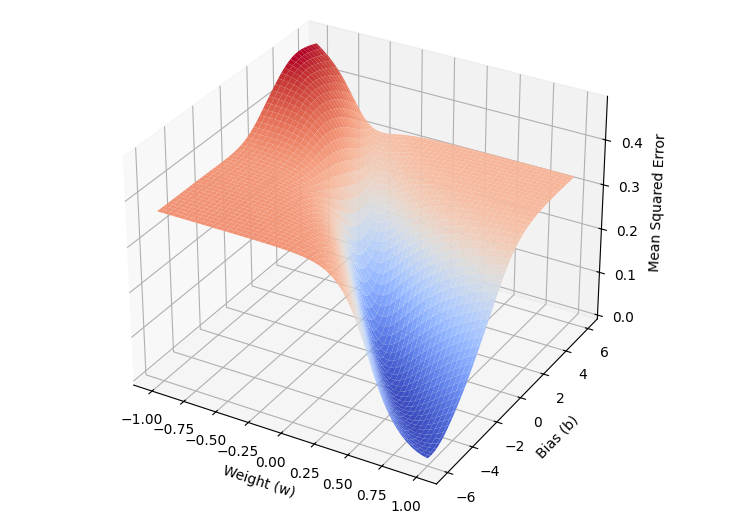
\includegraphics[width=0.7\textwidth]{content/section01/chapter01/figs/error_surface_sample.png}
    \caption{3D Error Surface Over Example Data}
    \label{fig:3d_error_example}
\end{figure}


\subsection{Sigmoid Neuron Learning Algorithm: Gradient Descent}

Let \( \boldsymbol{\theta} = [w, b] \) be the vector of parameters, initialized randomly. Suppose we move in the direction of a change \( \Delta \boldsymbol{\theta} = [\Delta w, \Delta b] \). Instead of making a full step, we scale the movement by a small scalar \( \eta \) to stay conservative. 
\[
\boldsymbol{\theta}_{\text{new}} = \boldsymbol{\theta} + \eta \cdot \Delta \boldsymbol{\theta}
\]

\textit{What is the right \( \Delta \boldsymbol{\theta} \) to choose?}
To answer this, we turn to the Taylor series expansion. Let \( \boldsymbol{u} = \Delta \boldsymbol{\theta} \). Then the Taylor expansion of the loss function \( \mathcal{L}(\boldsymbol{\theta}) \) around \( \boldsymbol{\theta} \) is 
\[
\mathcal{L}(\boldsymbol{\theta} + \eta \boldsymbol{u}) = \mathcal{L}(\boldsymbol{\theta}) + \eta \cdot \boldsymbol{u}^T \nabla_{\boldsymbol{\theta}} \mathcal{L}(\boldsymbol{\theta}) + \frac{\eta^2}{2!} \cdot \boldsymbol{u}^T \nabla^2 \mathcal{L}(\boldsymbol{\theta}) \boldsymbol{u} + \frac{\eta^3}{3!} \cdot \ldots
\]
Since \( \eta \) is small, the higher-order terms are negligible.
\[
\mathcal{L}(\boldsymbol{\theta} + \eta \boldsymbol{u}) \approx \mathcal{L}(\boldsymbol{\theta}) + \eta \cdot \boldsymbol{u}^T \nabla_{\boldsymbol{\theta}} \mathcal{L}(\boldsymbol{\theta})
\]
For the move to reduce the loss, we require
\[
\mathcal{L}(\boldsymbol{\theta} + \eta \boldsymbol{u}) - \mathcal{L}(\boldsymbol{\theta}) < 0 \quad \Rightarrow \quad \boldsymbol{u}^T \nabla_{\boldsymbol{\theta}} \mathcal{L}(\boldsymbol{\theta}) < 0
\]
To understand how negative this term can be, consider the angle \( \beta \) between \( \boldsymbol{u} \) and \( \nabla_{\boldsymbol{\theta}} \mathcal{L}(\boldsymbol{\theta}) \). 
\[
\cos(\beta) = \frac{\boldsymbol{u}^T \nabla_{\boldsymbol{\theta}} \mathcal{L}(\boldsymbol{\theta})}{\|\boldsymbol{u}\| \cdot \| \nabla_{\boldsymbol{\theta}} \mathcal{L}(\boldsymbol{\theta}) \|} \text{ and } -1 \leq \cos(\beta) \leq 1
\]
Let \( k = \|\boldsymbol{u}\| \cdot \|\nabla_{\boldsymbol{\theta}} \mathcal{L}(\boldsymbol{\theta})\| \), then
\[
-k \leq \boldsymbol{u}^T \nabla_{\boldsymbol{\theta}} \mathcal{L}(\boldsymbol{\theta}) \leq k
\]
This implies that the most negative value is attained when \( \cos(\beta) = -1 \), i.e., when the angle is 180°.
\[
\boldsymbol{u} = -\nabla_{\boldsymbol{\theta}} \mathcal{L}(\boldsymbol{\theta})
\]

Hence, the \textit{gradient descent rule} says that the direction \( \boldsymbol{u} \) to move in should be opposite to the gradient of the loss.
\[
w_{t+1} = w_t - \eta \frac{\partial \mathcal{L}(w, b)}{\partial w}\bigg|_{w = w_t, b = b_t}
\quad \text{and} \quad
b_{t+1} = b_t - \eta \frac{\partial \mathcal{L}(w, b)}{\partial b}\bigg|_{w = w_t, b = b_t}
\]

\begin{algobox}{Gradient Descent Algorithm}
\( t \gets 0 \) \\
max iterations \( \gets 1000 \) \\
\textbf{while} \( t < \) max iterations \textbf{do} \\
\hspace*{1em} \( w_{t+1} \gets w_t - \eta \nabla_w \mathcal{L}(w_t, b_t) \) \\
\hspace*{1em} \( b_{t+1} \gets b_t - \eta \nabla_b \mathcal{L}(w_t, b_t) \) \\
\hspace*{1em} \( t \gets t + 1 \) \\
\textbf{end while}
\end{algobox}

Starting from initial values \( w = 0 \) and \( b = 0 \), gradient descent converges to final parameters \( w = 0.1487 \), \( b = -0.4139 \) with a final loss of \( 0.0527 \) after 100 iterations.\newpage

\begin{figure}[h!]
    \centering
    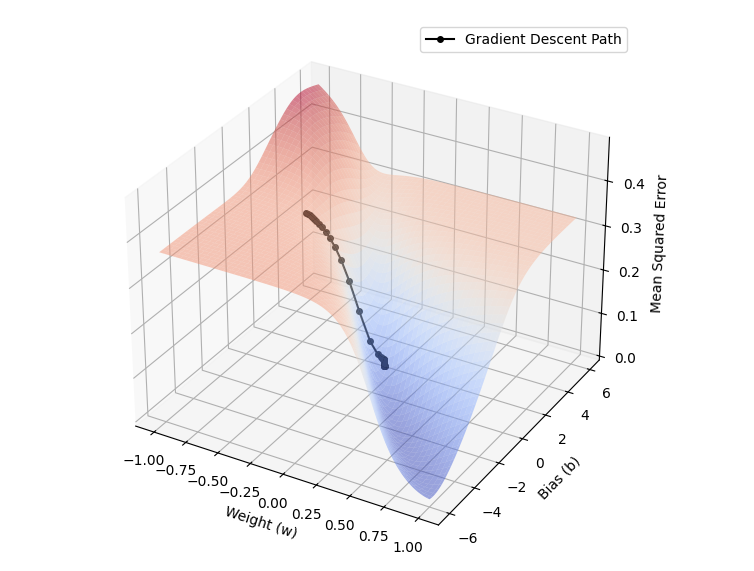
\includegraphics[width=0.7\textwidth]{content/section01/chapter01/figs/error_surface_grad_desc.png}
    \caption{Error Surface With Gradient Descent Trajectory.}
    \label{fig:gd_trajectory}
\end{figure}

\begin{figure}[h!]
    \centering
    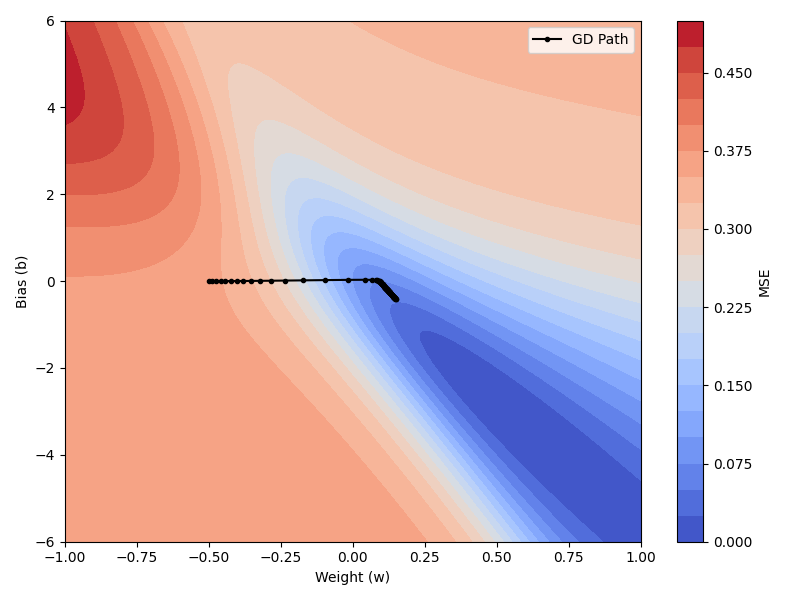
\includegraphics[width=0.65\textwidth]{content/section01/chapter01/figs/grad_desc_contour.png}
    \caption{Contour Plot of Gradient Descent Trajectory on Error Surface.}
\end{figure}

Visualizing in three dimensions can get cumbersome. So, we use 2D contour plots instead.  When the contours are close together, the slope is steep in that direction.  


\subsection{Momentum Based Gradient Descent}

Gradient descent can be slow in regions with gentle slopes. This happens because the gradient becomes very small, leading to small updates. To improve this, we can look at how updates behave over time.

The intuition is that if we keep getting asked to move in the same direction, it's reasonable to trust that direction and take bigger steps --- just like a ball gathers speed when rolling downhill.
\[
\text{update}_t = \gamma \cdot \text{update}_{t-1} + \eta \nabla w_t  
\]
\[
w_{t+1} = w_t - \text{update}_t
\]
Here, $\gamma$ is the momentum coefficient (typically between 0.5 and 0.9), and $\eta$ is the learning rate. This rule incorporates both the current gradient and the accumulated history of past gradients.
\begin{align*}
\text{update}_0 &= 0 \\
\text{update}_1 &= \gamma \cdot \text{update}_0 + \eta \nabla w_1 = \eta \nabla w_1 \\
\text{update}_2 &= \gamma \cdot \text{update}_1 + \eta \nabla w_2 = \gamma \cdot \eta \nabla w_1 + \eta \nabla w_2 \\
\text{update}_3 &= \gamma \cdot \text{update}_2 + \eta \nabla w_3 = \gamma^2 \cdot \eta \nabla w_1 + \gamma \cdot \eta \nabla w_2 + \eta \nabla w_3 \\
\text{update}_4 &= \gamma \cdot \text{update}_3 + \eta \nabla w_4 = \gamma^3 \cdot \eta \nabla w_1 + \gamma^2 \cdot \eta \nabla w_2 + \gamma \cdot \eta \nabla w_3 + \eta \nabla w_4
\end{align*}

Continuing this process, we can write the general form, 
\[
\text{update}_t = \sum_{k=1}^{t} \gamma^{\text{ }t-k} \cdot \eta \nabla w_k
\] 
This shows that updates are a weighted sum of all past gradients, with exponentially decaying weights controlled by $\gamma$.

\begin{algobox}{Momentum-based Gradient Descent Algorithm}
\( t \gets 0 \) \\
max iterations \( \gets 1000 \) \\
initialize updates: \( u^w_0 \gets 0, \quad u^b_0 \gets 0 \) \\
momentum coefficient \( \gamma \in [0,1) \) \\
learning rate \( \eta > 0 \) \\
\textbf{while} \( t < \) max iterations \textbf{do} \\
\hspace*{1em} \( u^w_{t+1} \gets \gamma \cdot u^w_t + \eta \nabla_w \mathcal{L}(w_t, b_t) \) \\
\hspace*{1em} \( u^b_{t+1} \gets \gamma \cdot u^b_t + \eta \nabla_b \mathcal{L}(w_t, b_t) \) \\
\hspace*{1em} \( w_{t+1} \gets w_t - u^w_{t+1} \) \\
\hspace*{1em} \( b_{t+1} \gets b_t - u^b_{t+1} \) \\
\hspace*{1em} \( t \gets t + 1 \) \\
\textbf{end while}
\end{algobox}


\begin{figure}[h!]
    \centering
    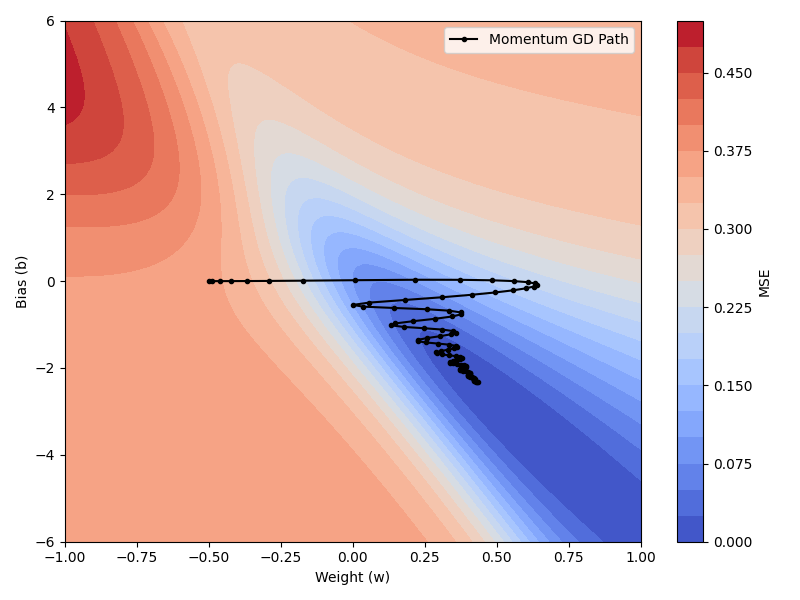
\includegraphics[width=0.65\textwidth]{content/section01/chapter01/figs/momentum_grad_desc_contour.png}
    \caption{Contour Plot of Momentum Gradient Descent Trajectory on Error Surface.}
\end{figure}

In our example, consider the initial values \( w = 0 \) and \( b = 0 \) and $\gamma = 0.9$. Momentum gradient descent converges to final parameters \( w = 0.4328 \), \( b = -2.3303 \) with a final loss of \( 0.004201 \) after 100 iterations. This surely performs better than the vanilla gradient descent. 

\subsection{Nesterov Accelerated Gradient Descent}

Even in regions with gentle slopes, momentum-based gradient descent takes large steps because momentum carries it forward. It oscillates in and out of the minima valley, often taking many U-turns before finally converging. Despite these oscillations, it converges faster than vanilla gradient descent. But \textit{can we reduce these oscillations?}

The intuition is to \textit{look before we leap}. Recall the momentum update equation,
\[
\text{update}_t = \gamma \cdot \text{update}_{t-1} + \eta \nabla_w \mathbf{w}_t
\]
We move at least by \(\gamma \cdot \text{update}_{t-1}\), plus a bit more by \(\eta \nabla_w \mathbf{w}_t\).

\textit{What if we calculate the gradient at a look-ahead point instead of the current position?} Let's say we define
\[
\mathbf{w}_{\text{look ahead}} = \mathbf{w}_t - \gamma \cdot \text{update}_{t-1}
\]
Then calculate the gradient \(\nabla_w \mathbf{w}_{\text{look ahead}}\) instead of \(\nabla_w \mathbf{w}_t\).

Thus, the update rule for Nesterov Accelerated Gradient (NAG) becomes
\[
\begin{aligned}
\mathbf{w}_{\text{look ahead}} &= \mathbf{w}_t - \gamma \cdot \text{update}_{t-1} \\
\text{update}_t &= \gamma \cdot \text{update}_{t-1} + \eta \nabla_w \mathbf{w}_{\text{look ahead}} \\
\mathbf{w}_{t+1} &= \mathbf{w}_t - \text{update}_t
\end{aligned}
\]

A similar update applies for the bias term \(b_t\).

\begin{algobox}{Nesterov Accelerated Gradient (NAG) Algorithm}
\( t \gets 0 \) \\
max iterations \( \gets 1000 \) \\
initialize \( \text{update}^w_{-1} \gets \mathbf{0} \), \( \text{update}^b_{-1} \gets 0 \) \\
momentum coefficient \( \gamma \in [0,1) \) \\
learning rate \( \eta > 0 \) \\

\textbf{while} \( t < \) max iterations \textbf{do} \\
\hspace*{1em} \(\mathbf{w}_{\text{look ahead}} \gets \mathbf{w}_t - \gamma \cdot \text{update}^w_{t-1}\) \\
\hspace*{1em} \(b_{\text{look ahead}} \gets b_t - \gamma \cdot \text{update}^b_{t-1}\) \\

\hspace*{1em} \(\text{update}^w_t \gets \gamma \cdot \text{update}^w_{t-1} + \eta \nabla_w \mathcal{L}(\mathbf{w}_{\text{look ahead}}, b_{\text{look ahead}})\) \\
\hspace*{1em} \(\text{update}^b_t \gets \gamma \cdot \text{update}^b_{t-1} + \eta \nabla_b \mathcal{L}(\mathbf{w}_{\text{look ahead}}, b_{\text{look ahead}})\) \\

\hspace*{1em} \(\mathbf{w}_{t+1} \gets \mathbf{w}_t - \text{update}^w_t\) \\
\hspace*{1em} \(b_{t+1} \gets b_t - \text{update}^b_t\) \\
\hspace*{1em} \( t \gets t + 1 \) \\
\textbf{end while}
\end{algobox}

\begin{figure}[h!]
    \centering
    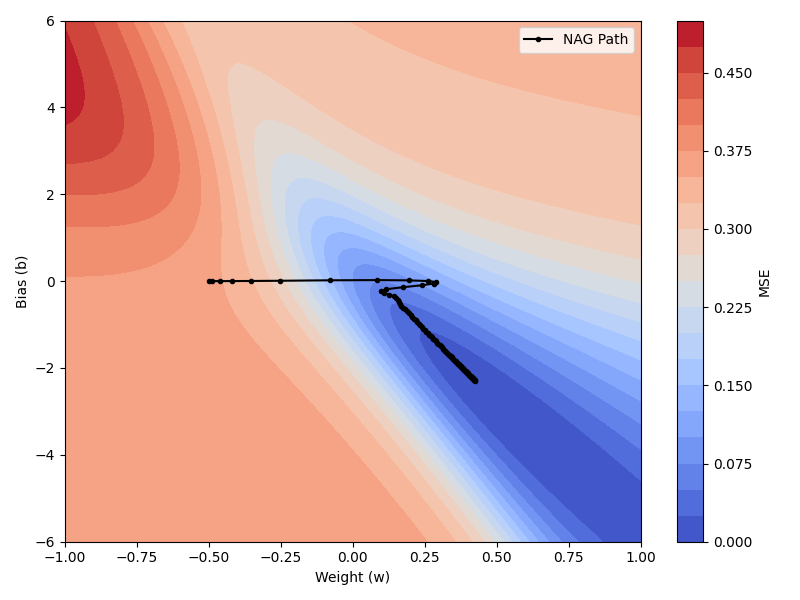
\includegraphics[width=0.65\textwidth]{content/section01/chapter01/figs/nesterov_grad_desc_contour.png}
    \caption{Contour Plot of Nesterov Gradient Descent Trajectory on Error Surface.}
\end{figure}

Looking ahead allows NAG to correct its course faster than momentum-based gradient descent. This reduces oscillations and lowers the chance of escaping the minima valley.

Starting from initial values \( w = 0 \) and \( b = 0 \), Nesterov Gradient Descent converges to final parameters \( w = 0.4247 \), \( b = -2.2946 \) with a final loss of \( 0.004477 \) after 100 iterations.

\subsection{Stochastic Gradient Descent}

Batch gradient descent computes the exact gradient of the loss by averaging the gradients over the entire dataset before updating the parameters. Because the full dataset is used, each update guarantees a decrease in the loss. 

However, this method becomes computationally expensive for large datasets. For example, with one million data points, one parameter update requires calculating one million gradients.

Stochastic Gradient Descent (SGD) improves efficiency by updating parameters after evaluating the gradient on each individual data point. Hence, for one million data points, SGD performs one million updates per epoch, where an \emph{epoch} is defined as a full pass over the dataset.

However, the gradient used in SGD is a noisy, stochastic estimate of the true gradient since it is computed using only one data point rather than the entire dataset. Due to this noise, there is no guarantee that each SGD update reduces the overall loss function. Indeed, the updates tend to oscillate, especially in small datasets, as each data point tries to optimize locally without considering the global effect on other points.

Even with these jumps, SGD can still find a good solution in the long run, as long as the learning rate is adjusted properly over time.

To smooth things out, we can use mini-batches. Instead of just one point, we use a small group of data points to compute the gradient. This reduces the noise while keeping the updates fast. It also helps the model converge more smoothly.

Also, the randomness in SGD isn’t always bad. It can help the model escape flat spots or shallow traps in the loss surface, which sometimes leads to better results.



\begin{algobox}{Mini-Batch Stochastic Gradient Descent Algorithm}
\( t \gets 0 \) \\
max iterations \( \gets 1000 \) \\
mini-batch size \( \gets m \) \\

\textbf{while} \( t < \) max iterations \textbf{do} \\
\hspace*{1em} Sample mini-batch \( \mathcal{B}_t \) of size \( m \) from training data \\

\hspace*{1em} Compute gradients over mini-batch: \\
\hspace*{2em} \( g_w \gets \frac{1}{m} \sum_{(x_i,y_i) \in \mathcal{B}_t} \nabla_w \mathcal{L}(w_t, b_t; \text{ }x_i, y_i) \) \\
\hspace*{2em} \( g_b \gets \frac{1}{m} \sum_{(x_i,y_i) \in \mathcal{B}_t} \nabla_b \mathcal{L}(w_t, b_t; \text{ }x_i, y_i) \) \\

\hspace*{2em} \( w_{t+1} \gets w_t - \eta g_w \) \\
\hspace*{2em} \( b_{t+1} \gets b_t - \eta g_b \) \\

\hspace*{1em} \( t \gets t + 1 \) \\
\textbf{end while}
\end{algobox}

Starting from initial values \( w = 0 \) and \( b = 0 \), Stochastic Gradient Descent converges to final parameters \( w = 0.3706 \), \( b = -1.9689 \) with a final loss of \( 0.007861 \) after 100 iterations.

\begin{figure}[h!]
    \centering
    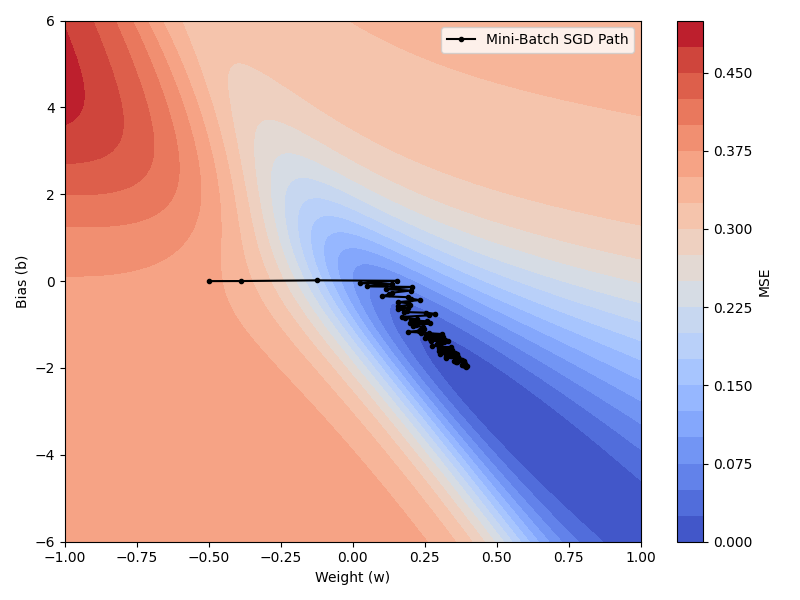
\includegraphics[width=0.65\textwidth]{content/section01/chapter01/figs/sgd_contour.png}
    \caption{Contour Plot of Stochastic Gradient Descent Trajectory on Error Surface.}
\end{figure}


\subsection{Gradient Descent with Adaptive Learning}

One might think to solve the problem of navigating gentle slopes by setting a high learning rate \( \eta \), effectively amplifying small gradients. But it is better to have a learning rate that adapts to the gradient itself.

\textbf{Intuition 1 (Adagrad):} Decay the learning rate for each parameter based on its past updates. More updates lead to more decay. The update rule for Adagrad is
\[
v_t = v_{t-1} + (\nabla w_t)^2
\]
\[
w_{t+1} = w_t - \frac{\eta}{\sqrt{v_t} + \epsilon} \cdot \nabla w_t
\]
A similar set of equations applies for the bias parameter \( b_t \).

\begin{algobox}{Batch Gradient Descent with Adagrad}
\( t \gets 0 \) , max iterations \( \gets 1000 \) \\
\( v_w \gets 0 \), \( v_b \gets 0 \) \\
\textbf{while} \( t < \) max iterations \textbf{do} \\
\hspace*{1em} \( g_{w_t} \gets \nabla_w \mathcal{L}(w_t, b_t) \) , \quad \( g_{b_t} \gets \nabla_b \mathcal{L}(w_t, b_t) \) \\
\hspace*{1em} \( v_w \gets v_w + g_{w_t}^2 \) , \quad \( v_b \gets v_b + g_{b_t}^2 \) \\
\hspace*{1em} \( w_{t+1} \gets w_t - \frac{\eta}{\sqrt{v_w} + \epsilon} \cdot g_{w_t} \) , \quad \( b_{t+1} \gets b_t - \frac{\eta}{\sqrt{v_b} + \epsilon} \cdot g_{b_t} \) \\
\hspace*{1em} \( t \gets t + 1 \) \\
\textbf{end while}
\end{algobox}


\begin{figure}[h!]
    \centering
    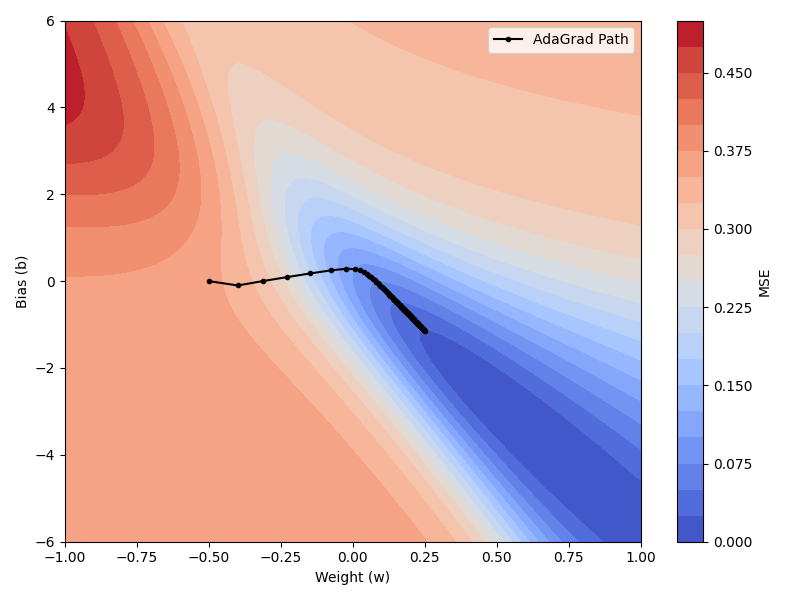
\includegraphics[width=0.65\textwidth]{content/section01/chapter01/figs/adagrad_gd_contour.png}
    \caption{Contour Plot of Gradient Descent Trajectory with Adagrad Learning on Error Surface.}
\end{figure}

Starting from initial values \( w = 0 \) and \( b = 0 \), Gradient Descent with Adagrad Learning converges to final parameters \( w = 0.2493 \), \( b = -1.1415 \) with a final loss of \( 0.024577 \) after 100 iterations.


\textbf{Intuition 2 (RMSProp):} Adagrad decays the learning rate too aggressively. After some time, frequently updated parameters get very small updates because the denominator \( \sqrt{v_t} \) grows without bound. To fix this, RMSProp decays \( v_t \) to prevent its rapid growth.

The update rule for RMSProp is
\[
v_t = \beta \cdot v_{t-1} + (1 - \beta) \cdot (\nabla w_t)^2
\]
\[
w_{t+1} = w_t - \frac{\eta}{\sqrt{v_t} + \epsilon} \cdot \nabla w_t
\]
Again, a similar set of equations applies for \( b_t \).

\begin{algobox}{Batch Gradient Descent with RMSProp}
\( t \gets 0 \) , max iterations \( \gets 1000 \) \\
Initialize \( v_w \gets 0 \), \( v_b \gets 0 \) \\
Choose \( \eta, \beta, \epsilon \) \\
\textbf{while} \( t < \) max iterations \textbf{do} \\
\hspace*{1em} \( g_w \gets \nabla_w \mathcal{L}(w_t, b_t) \),\quad \( g_b \gets \nabla_b \mathcal{L}(w_t, b_t) \) \\
\hspace*{1em} \( v_w \gets \beta \cdot v_w + (1 - \beta) \cdot g_w^2 \) , \quad \( v_b \gets \beta \cdot v_b + (1 - \beta) \cdot g_b^2 \) \\
\hspace*{1em} \( w_{t+1} \gets w_t - \frac{\eta}{\sqrt{v_w} + \epsilon} \cdot g_w \) , \quad \( b_{t+1} \gets b_t - \frac{\eta}{\sqrt{v_b} + \epsilon} \cdot g_b \) \\
\hspace*{1em} \( t \gets t + 1 \) \\
\textbf{end while}
\end{algobox}


Adagrad gets stuck near convergence because its learning rate decays too much, making it hard to move in some directions (like the vertical \( b \) direction). RMSProp fixes this by decaying \( v_t \) less aggressively.

\begin{figure}[h!]
    \centering
    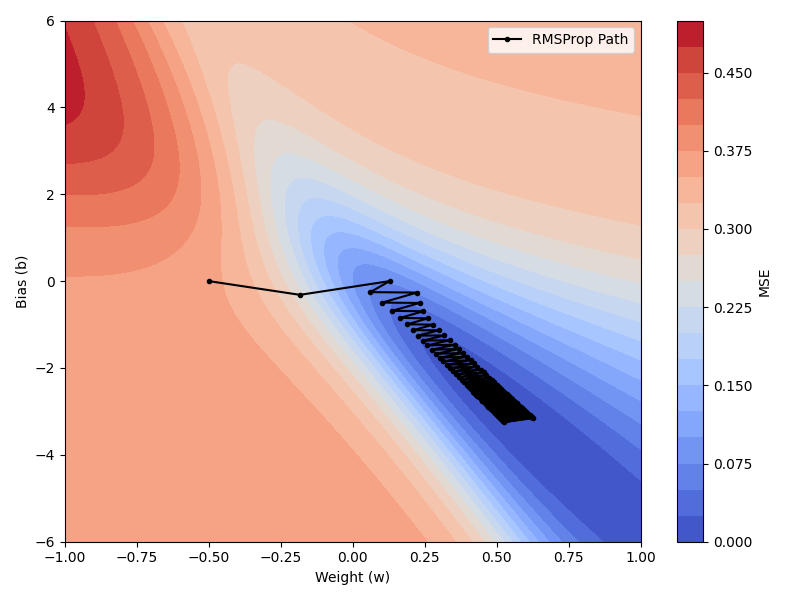
\includegraphics[width=0.7\textwidth]{content/section01/chapter01/figs/rmsprop_gd_contour.png}
    \caption{Contour Plot of Gradient Descent Trajectory with RMSProp Learning on Error Surface.}
\end{figure}

Starting from initial values \( w = 0 \) and \( b = 0 \), Gradient Descent with RMSProp Learning converges to final parameters \( w = 0.6249 \), \( b = -3.1551 \) with a final loss of \( 0.005095 \) after 100 iterations.

\textbf{Intuition 3 (Adam):} Adam builds on RMSProp by also keeping a cumulative history of gradients (first moment estimate).

The update rules for Adam are
\[
m_t = \beta_1 \cdot m_{t-1} + (1 - \beta_1) \cdot \nabla w_t
\]
\[
v_t = \beta_2 \cdot v_{t-1} + (1 - \beta_2) \cdot (\nabla w_t)^2
\]
\[
\hat{m}_t = \frac{m_t}{1 - \beta_1^t}
\]
\[
\hat{v}_t = \frac{v_t}{1 - \beta_2^t}
\]
\[
w_{t+1} = w_t - \frac{\eta}{\sqrt{\hat{v}_t} + \epsilon} \cdot \hat{m}_t
\]

A similar set of equations applies for \( b_t \).

Starting from initial values \( w = 0 \) and \( b = 0 \), Gradient Descent with Adam Learning converges to final parameters \( w = 0.5227 \), \( b = -2.9403 \) with a final loss of \( 0.001289 \) after 100 iterations.

\begin{algobox}{Batch Gradient Descent with Adam}
\( t \gets 0 \)  , \quad max iterations \( \gets 1000 \) \\
Initialize \( m_w = 0, \; v_w = 0, \; m_b = 0, \; v_b = 0 \) \\
Choose \(\beta_1, \beta_2\) \\

\textbf{while} \( t < \) max iterations \textbf{do} \\
\hspace*{1em} Compute gradients: \( g_w \gets \nabla_w \mathcal{L}(w_t, b_t) \), \( g_b \gets \nabla_b \mathcal{L}(w_t, b_t) \) \\

\hspace*{1em} \( m_w \gets \beta_1 \cdot m_w + (1 - \beta_1) \cdot g_w \) , \quad \( v_w \gets \beta_2 \cdot v_w + (1 - \beta_2) \cdot g_w^2 \) \\
\hspace*{1em} \( \hat{m}_w \gets \frac{m_w}{1 - \beta_1^t} \) , \quad \( \hat{v}_w \gets \frac{v_w}{1 - \beta_2^t} \) \\
\hspace*{1em} \( w_{t+1} \gets w_t - \frac{\eta}{\sqrt{\hat{v}_w} + \epsilon} \cdot \hat{m}_w \) \\

\hspace*{1em} \( m_b \gets \beta_1 \cdot m_b + (1 - \beta_1) \cdot g_b \) , \quad \( v_b \gets \beta_2 \cdot v_b + (1 - \beta_2) \cdot g_b^2 \) \\
\hspace*{1em} \( \hat{m}_b \gets \frac{m_b}{1 - \beta_1^t} \) , \quad \( \hat{v}_b \gets \frac{v_b}{1 - \beta_2^t} \) \\
\hspace*{1em} \( b_{t+1} \gets b_t - \frac{\eta}{\sqrt{\hat{v}_b} + \epsilon} \cdot \hat{m}_b \) \\

\hspace*{1em} \( t \gets t + 1 \) \\
\textbf{end while}
\end{algobox}


\begin{figure}[h!]
    \centering
    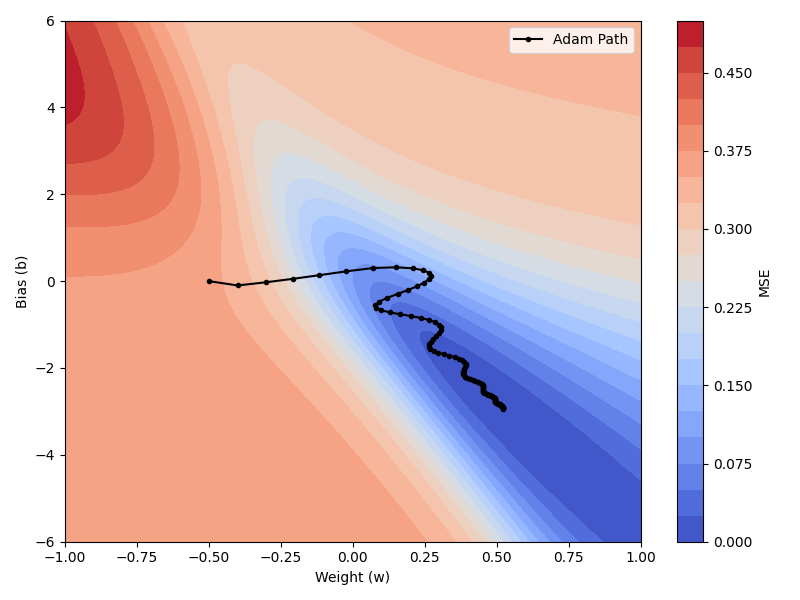
\includegraphics[width=0.7\textwidth]{content/section01/chapter01/figs/adam_gd_contour.png}
    \caption{Contour Plot of Gradient Descent Trajectory with Adam Learning on Error Surface.}
\end{figure}

All these adaptive learning rate methods modify the vanilla gradient descent update. Adam can also be combined with Nesterov's lookahead method for further improvements.

\begin{algobox}{Nesterov-Adam (Nadam) Algorithm}
\( t \gets 0 \), \quad max iterations \( \gets 1000 \) \\
Initialize \( m_w = 0, \; v_w = 0, \; m_b = 0, \; v_b = 0 \) \\
Initialize \( w_0, \; b_0 \), \quad momentum coefficient \( \gamma = \beta_1 \in [0,1) \), \quad learning rate \( \eta > 0 \) \\
\textbf{while} \( t < \) max iterations \textbf{do} \\
\hspace*{1em} \( \mathbf{w}_{\text{look ahead}} \gets \mathbf{w}_t - \gamma \cdot m_w \) \\
\hspace*{1em} \( b_{\text{look ahead}} \gets b_t - \gamma \cdot m_b \) \\
\hspace*{1em} Compute gradients: \( g_w \gets \nabla_w \mathcal{L}(\mathbf{w}_{\text{look ahead}}, b_{\text{look ahead}}) \), \quad \( g_b \gets \nabla_b \mathcal{L}(\mathbf{w}_{\text{look ahead}}, b_{\text{look ahead}}) \) \\

\hspace*{1em} \( m_w \gets \beta_1 \cdot m_w + (1 - \beta_1) \cdot g_w \) , \quad \( v_w \gets \beta_2 \cdot v_w + (1 - \beta_2) \cdot g_w^2 \) \\
\hspace*{1em} \( \hat{m}_w \gets \frac{m_w}{1 - \beta_1^{t+1}} \) , \quad \( \hat{v}_w \gets \frac{v_w}{1 - \beta_2^{t+1}} \) \\
\hspace*{1em} \( w_{t+1} \gets w_t - \frac{\eta}{\sqrt{\hat{v}_w} + \epsilon} \cdot (\gamma \cdot \hat{m}_w + (1 - \gamma) \cdot g_w) \) \\

\hspace*{1em} \( m_b \gets \beta_1 \cdot m_b + (1 - \beta_1) \cdot g_b \) , \quad \( v_b \gets \beta_2 \cdot v_b + (1 - \beta_2) \cdot g_b^2 \) \\
\hspace*{1em} \( \hat{m}_b \gets \frac{m_b}{1 - \beta_1^{t+1}} \) , \quad \( \hat{v}_b \gets \frac{v_b}{1 - \beta_2^{t+1}} \) \\
\hspace*{1em} \( b_{t+1} \gets b_t - \frac{\eta}{\sqrt{\hat{v}_b} + \epsilon} \cdot (\gamma \cdot \hat{m}_b + (1 - \gamma) \cdot g_b) \) \\
\hspace*{1em} \( t \gets t + 1 \) \\
\textbf{end while}
\end{algobox}


\begin{figure}[h!]
    \centering
    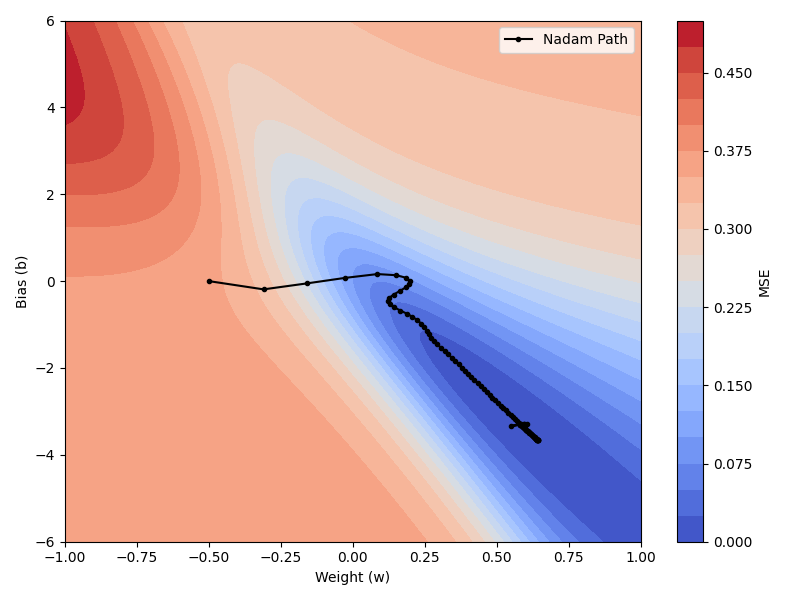
\includegraphics[width=0.7\textwidth]{content/section01/chapter01/figs/nadam.png}
    \caption{Contour Plot of Nesterov Gradient Descent Trajectory with Adam Learning on Error Surface.}
\end{figure}

Starting from initial values \( w = 0 \) and \( b = 0 \), Nesterov Gradient Descent with Adam Learning converges to final parameters \( w = 0.5829 \), \( b = -3.3043 \) with a final loss of \( 0.000833 \) after 100 iterations.

\begin{table}[h!]
\centering
\begin{tabular}{|l|c|c|c|}
\hline
\textbf{Method} & \textbf{Final Parameters (w, b)} & \textbf{Final Loss} \\ \hline
Vanilla Gradient Descent & \( w = 0.1487,\; b = -0.4139 \) & 0.0527 \\ \hline
Momentum Gradient Descent (\( \gamma = 0.9 \)) & \( w = 0.4328,\; b = -2.3303 \) & 0.004201 \\ \hline
Nesterov Gradient Descent & \( w = 0.4247,\; b = -2.2946 \) & 0.004477 \\ \hline
Stochastic Gradient Descent & \( w = 0.3706,\; b = -1.9689 \) & 0.007861 \\ \hline
Adagrad Gradient Descent & \( w = 0.2493,\; b = -1.1415 \) & 0.024577 \\ \hline
RMSProp Gradient Descent & \( w = 0.6249,\; b = -3.1551 \) & 0.005095 \\ \hline
Adam Gradient Descent & \( w = 0.5227,\; b = -2.9403 \) & 0.001289 \\ \hline
\textbf{Nesterov with Adam (Best)} & \textbf{\( w = 0.5829,\; b = -3.3043 \)} & \textbf{0.000833} \\ \hline
\end{tabular}
\caption{Comparison of Gradient Descent Methods (Initial values: \( w = 0 \), \( b = 0 \), 100 iterations)}
\end{table}


\subsection{Layer of Sigmoid Neurons}

Recall a multilayer network of perceptrons with a single hidden layer can be used to represent any boolean function precisely (no errors). Similarly, the representation power of a multilayer network of sigmoid neurons is given by the \textbf{Universal Approximation Theorem.} To prove this, we will need the result from \textbf{Stone-Weierstrass Theorem}. 

\begin{theorem}
    \label{thm:stone-weierstrass}
    \textbf{Stone-Weierstrass Theorem}. Let $K$ be a compact subset of $\mathbb{R}^n$ and let $\mathcal{A}$ be a subalgebra of $C(K)$ (the space of continuous real-valued functions on $K$) such that 
\begin{enumerate}
    \item $\mathcal{A}$ separates points of $K$ (i.e., for any $x, y \in K$ with $x \neq y$, there exists $f \in \mathcal{A}$ such that $f(x) \neq f(y)$)
    \item $\mathcal{A}$ contains the constant functions
\end{enumerate}
Then $\mathcal{A}$ is dense in $C(K)$ with respect to the uniform norm.
\end{theorem}

Imagine you have a collection of continuous functions defined on a \textit{nice} and \textit{closed} space (like a closed and bounded interval). If this collection of functions has two key properties:
\begin{enumerate}
    \item \textit{They can tell points apart}. For any two distinct points in your space, you can find a function in your collection that gives different values for those two points.
    \item \textit{They include all the constant functions}. You have functions in your collection that are just a fixed number everywhere.
\end{enumerate}
Then, you can use combinations of these functions (adding them, multiplying them, multiplying them by constants) to get arbitrarily close to any other continuous function on that space.

Essentially, if your initial collection of functions is rich enough to distinguish between points and includes constants, it's \textit{dense} enough to build approximations for any other continuous function you can think of on that space.

\begin{proof}
Let \( f \in C(K) \) and \( \varepsilon > 0 \). We aim to show that there exists a function \( g \in \mathcal{A} \) such that 
\[
\|f - g\|_\infty < \varepsilon.
\]

\textbf{Step 1: Approximate indicator functions.}

Fix \( x_0 \in K \). For any \( x \in K \), since \( \mathcal{A} \) separates points, there exists \( \phi_x \in \mathcal{A} \) such that \( \phi_x(x) \neq \phi_x(x_0) \). Define:
\[
\psi_x(y) = \left( \frac{\phi_x(y) - \phi_x(x_0)}{\phi_x(x) - \phi_x(x_0)} \right)^2.
\]
Then \( \psi_x \in \mathcal{A} \) because \( \mathcal{A} \) is a subalgebra (closed under addition, multiplication, and scalar multiplication), and we’ve used only these operations. Also, \( \psi_x(x_0) = 0 \), and \( \psi_x(x) = 1 \).

Now, for a finite set \( \{x_1, \dots, x_m\} \subset K \), we can construct a partition of unity-like approximation by defining functions \( \{\psi_{x_j}\}_{j=1}^m \) and then normalize
\[
S(y) = \sum_{j=1}^m \psi_{x_j}(y), \quad \rho_j(y) = \frac{\psi_{x_j}(y)}{S(y)}.
\]
Each \( \rho_j \in \mathcal{A} \), and \( \sum_{j=1}^m \rho_j(y) = 1 \) for all \( y \in K \).

\textbf{Step 2: Local approximation of \( f \).}

Since \( f \) is uniformly continuous on compact \( K \), there exists a finite \( \delta \)-net \( \{x_1, \dots, x_m\} \subset K \) such that for all \( y \in K \), there exists \( x_j \) with \( |f(y) - f(x_j)| < \varepsilon \). 

Now define the function
\[
g(y) = \sum_{j=1}^m f(x_j) \rho_j(y).
\]
Then \( g \in \mathcal{A} \) because \( \rho_j \in \mathcal{A} \) and \( f(x_j) \) are constants (constants are in \( \mathcal{A} \), and the algebra is closed under scalar multiplication and addition).

\textbf{Step 3: Approximation bound.}

We estimate the uniform difference
\[
|f(y) - g(y)| = \left|f(y) - \sum_{j=1}^m f(x_j) \rho_j(y)\right| = \left|\sum_{j=1}^m \rho_j(y) (f(y) - f(x_j))\right|.
\]
Using the triangle inequality
\[
|f(y) - g(y)| \leq \sum_{j=1}^m \rho_j(y) |f(y) - f(x_j)|.
\]
Since each \( \rho_j(y) \geq 0 \), and \( \sum \rho_j(y) = 1 \), this is a convex combination of errors \( |f(y) - f(x_j)| \), each less than \( \varepsilon \). So,
\[
|f(y) - g(y)| < \varepsilon \quad \text{for all } y \in K.
\]
Hence,
\[
\|f - g\|_\infty < \varepsilon.
\]
\end{proof}

\begin{example}
    Polynomials can be used to approximate any continuous function on a closed interval.
\end{example}

\begin{solution}
Let $K$ be a compact subset of $\mathbb{R}^n$. We consider the subalgebra $\mathcal{A}$ of $C(K)$ consisting of all polynomial functions on $K$. For clarity, let's first consider the common case where $K$ is a closed and bounded interval in $\mathbb{R}$, say $K = [a, b]$.

A function $f \in \mathcal{A}$ has the form $f(x) = c_m x^m + c_{m-1} x^{m-1} + \dots + c_1 x + c_0$ for some non-negative integer $m$ and real coefficients $c_0, c_1, \dots, c_m$.

We need to demonstrate that $\mathcal{A}$ satisfies the two properties required by the Stone-Weierstrass Theorem.

\textbf{1. $\mathcal{A}$ separates points of $K$}

This property requires that for any distinct points $x, y \in K$ (i.e., $x \neq y$), there must exist a function $f \in \mathcal{A}$ such that $f(x) \neq f(y)$.

Consider any two distinct points $x, y \in [a, b]$ such that $x \neq y$.
Let's choose the polynomial function $f(t) = t$. This is a simple polynomial of degree 1 (where $m=1$, $c_1=1$, and $c_0=0$).
Evaluating this function at $x$ and $y$, we get $f(x) = x$ and $f(y) = y$.
Since we initially assumed $x \neq y$, it directly follows that $f(x) \neq f(y)$.

Therefore, the set of polynomial functions $\mathcal{A}$ successfully separates points of $K$.

\textbf{2. $\mathcal{A}$ contains the constant functions}

This property requires that for any real number $c$, the constant function $g(t) = c$ for all $t \in K$ must be an element of $\mathcal{A}$.

A constant function $g(t) = c$ can be expressed as a polynomial of degree 0. We can write $g(t) = c \cdot t^0$, or simply $g(t) = c$. This fits the general form of a polynomial where $m=0$ and $c_0=c$.

Thus, for any real number $c$, the constant function $g(t)=c$ is indeed a polynomial.

Therefore, the set of polynomial functions $\mathcal{A}$ contains all constant functions.

Since the set of polynomial functions on $K=[a,b]$ satisfies both of these crucial properties, the Stone-Weierstrass Theorem implies that the set of polynomials is \textbf{dense} in $C([a,b])$. 
\end{solution}

This is a fundamental result, meaning that any continuous real-valued function defined on a closed and bounded interval can be uniformly approximated arbitrarily well by polynomials. The argument extends naturally to compact subsets of $\mathbb{R}^n$. In this case, $\mathcal{A}$ would comprise polynomials in $n$ variables.


Refer figure \ref{fig:stone-weierstrass} for illustration.

\begin{figure}[h]
\centering
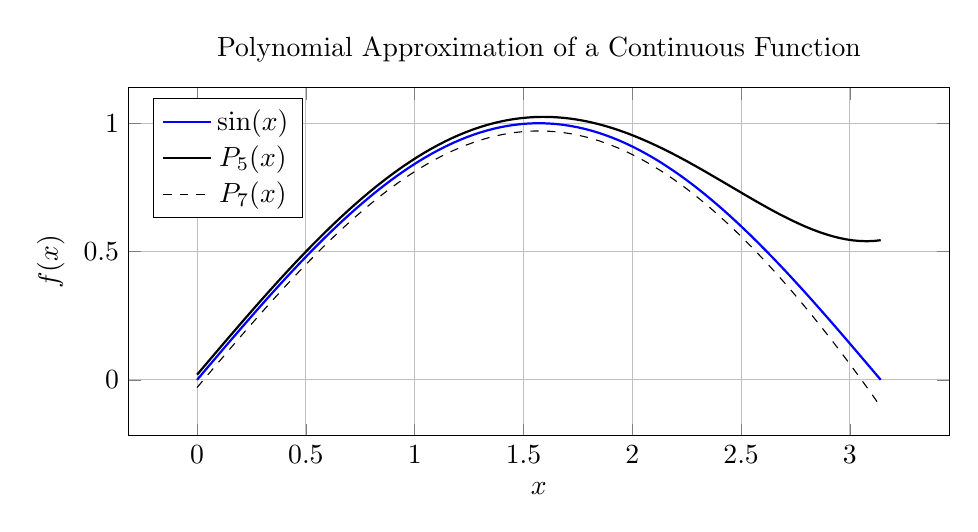
\begin{tikzpicture}
\begin{axis}[
    width=12cm,
    height=6cm,
    xlabel={$x$},
    ylabel={$f(x)$},
    title={Polynomial Approximation of a Continuous Function},
    grid=major,
    legend pos=north west,
    domain=0:pi,
    samples=100
]
\addplot[blue, thick] {sin(deg(x))};
\addplot[black, thick] {x - x^3/6 + x^5/120 + 0.02};
\addplot[black, dashed] {x - x^3/6 + x^5/120 - x^7/5040 - 0.03};
\legend{$\sin(x)$, $P_5(x)$, $P_7(x)$}
\end{axis}
\end{tikzpicture}
\caption{Illustration of the Stone-Weierstrass theorem. Polynomials $P_5(x)$ and $P_7(x)$ successively approximate $\sin(x)$ with increasing accuracy on the compact interval $[0, \pi]$.}
\label{fig:stone-weierstrass}
\end{figure}

\begin{theorem}
    \textbf{Universal Approximation Theorem.} Let $\sigma: \mathbb{R} \to \mathbb{R}$ be a non-constant, bounded, and continuous function (such as the sigmoid function). Let $K \subset \mathbb{R}^n$ be compact. Then for any continuous function $f: K \to \mathbb{R}$ and any $\varepsilon > 0$, there exist $N \in \mathbb{N}$, weights $\alpha_1, \ldots, \alpha_N \in \mathbb{R}$, weight vectors $\mathbf{w}_1, \ldots, \mathbf{w}_N \in \mathbb{R}^n$, and biases $b_1, \ldots, b_N \in \mathbb{R}$ such that the function
\[
g(\mathbf{x}) = \sum_{j=1}^{N} \alpha_j \sigma(\mathbf{w}_j^T \mathbf{x} + b_j)
\]
satisfies $\sup_{\mathbf{x} \in K} |f(\mathbf{x}) - g(\mathbf{x})| < \varepsilon$.
\end{theorem}

\begin{proof}
We want to show that the set of functions
\[
\mathcal{F} = \left\{ \sum_{j=1}^{N} \alpha_j \sigma(\mathbf{w}_j^T \mathbf{x} + b_j) : N \in \mathbb{N}, \text{ } \alpha_j \in \mathbb{R}, \text{ }\mathbf{w}_j \in \mathbb{R}^n, \text{ }b_j \in \mathbb{R} \right\}
\]
is dense in \( C(K) \), the space of continuous real-valued functions on compact \( K \subset \mathbb{R}^n \), with respect to the uniform norm.
Let us define
\[
\mathcal{A} = \text{span}\{ \sigma(\mathbf{w}^T \mathbf{x} + b) : \mathbf{w} \in \mathbb{R}^n, b \in \mathbb{R} \},
\]
which is a subalgebra of \( C(K) \). 

\textbf{Step 1: Closure under addition, multiplication, and scalar multiplication.}

The set \( \mathcal{A} \) is a linear span of compositions of affine functions with \( \sigma \), so it is closed under addition and scalar multiplication by construction. 

\textbf{Step 2: Separation of points.}

Let \( \mathbf{x}, \mathbf{y} \in K \) with \( \mathbf{x} \neq \mathbf{y} \). Since \( \sigma \) is non-constant and continuous, there exists a hyperplane (i.e., choice of \( \mathbf{w} \in \mathbb{R}^n \)) such that \( \mathbf{w}^T \mathbf{x} \neq \mathbf{w}^T \mathbf{y} \). Then for any fixed \( b \), we have
\[
\sigma(\mathbf{w}^T \mathbf{x} + b) \neq \sigma(\mathbf{w}^T \mathbf{y} + b),
\]
because \( \sigma \) is strictly increasing (as in sigmoid), or at least non-constant and continuous, so it distinguishes between different inputs. Hence, \( \mathcal{A} \) separates points of \( K \).

\textbf{Step 3: Constants are in \( \mathcal{A} \).}

Since \( \sigma \) is bounded and non-constant, it attains at least two values. For large positive or negative arguments, \( \sigma(z) \to c_1 \) or \( c_2 \), so we can scale and shift \( \sigma \) to approximate constant functions arbitrarily well. More directly, linear combinations of shifted sigmoids can approximate any constant function.
Hence, \( \mathcal{A} \) contains constant functions or can approximate them arbitrarily well, which is enough for density in the uniform norm.

By the Stone-Weierstrass Theorem~\ref{thm:stone-weierstrass}, \( \mathcal{A} \) is dense in \( C(K) \). Thus, for any \( f \in C(K) \) and \( \varepsilon > 0 \), there exists a finite sum of the form
\[
g(\mathbf{x}) = \sum_{j=1}^{N} \alpha_j \sigma(\mathbf{w}_j^T \mathbf{x} + b_j)
\]
such that
\[
\sup_{\mathbf{x} \in K} |f(\mathbf{x}) - g(\mathbf{x})| < \varepsilon.
\]
\end{proof}


\begin{corollary}
    A multilayer network of neurons with a single hidden layer can be used to approximate any continuous function to any desired precision. 
\end{corollary}

In other words, there is a guarantee that for any function \( f(\mathbf{x}) : \mathbb{R}^n \to \mathbb{R}^m \), we can always find a neural network (with one hidden layer containing enough sigmoid neurons) whose output \( g(\mathbf{x}) \) satisfies \( |g(\mathbf{x}) - f(\mathbf{x})| < \varepsilon \).

\section{Neural Network}

In earlier sections, we saw how a single layer of perceptrons or sigmoid neurons can represent any Boolean function or real function respectively. But there's a catch: the number of neurons needed grows exponentially with the number of inputs. That makes single-layer models impractical for real-world tasks.

Things changed in the 1980s. \textbf{\textit{Geoffrey Hinton}}, \textbf{\textit{David Rumelhart}}, and \textbf{\textit{Ronald Williams}} proposed a way to train networks with multiple hidden layers. Their work introduced the backpropagation algorithm \cite{rumelhart1986learning}, which made deep learning possible again. It allowed neural networks to be trained efficiently, layer by layer, even when stacked deep. This breakthrough helped revive interest in neural networks after a long period of disinterest in the field.

\subsection{Feedforward Neural Network Architecture}

We start with an input vector \( \mathbf{x} \in \mathbb{R}^n \), where \( n \) is the number of input features. This input passes through a sequence of layers in the network. A typical feedforward neural network has \( L \) layers in total, \( L - 1 \) hidden layers and one output layer.

Each hidden layer contains a certain number of neurons (often close to \( n \)), and every layer performs a transformation on the input it receives from the previous layer. For instance, \( L = 3 \) in figure \ref{fig:feedforward_nn}, as we have two hidden layers followed by an output layer.

\textbf{Structure of a Neuron}

Each neuron in the hidden and output layers operates in two steps:
\vspace{-5pt}
\begin{itemize}
    \item \textbf{\textit{Pre-activation:}} This is a linear transformation of the input from the previous layer. It combines the inputs using weights and adds a bias term. For the \( i^{\text{th}} \) layer, we denote this intermediate result by \( \mathbf{a}^{(i)} \in \mathbb{R}^n \).
    
    \item \textbf{\textit{Activation:}} This is a non-linear transformation of the pre-activation. The output is denoted by \( \mathbf{h}^{(i)} \in \mathbb{R}^n \).
\end{itemize}

This split into pre-activation and activation helps separate the roles of the linear and non-linear parts of the computation. The linear step captures how inputs are combined, while the non-linear step introduces flexibility. Without non-linearity, the entire network would collapse into a single linear transformation, no matter how many layers we stack.

Functions like sigmoid, tanh, and ReLU are used as activation functions. These functions are chosen because they are simple, differentiable, and behave differently for different inputs. This helps the network respond in varied ways, which is essential for learning complex patterns from data.

\begin{figure}[h!]
    \centering
    \def\layersep{3.5cm}

    \begin{tikzpicture}[shorten >=1pt,->,draw=black!50, node distance=\layersep]
        \tikzstyle{neuron}=[circle, minimum size=30pt, inner sep=0pt, draw=black]
        \tikzstyle{input neuron}=[neuron, fill=green!30, opacity=0.6]
        \tikzstyle{hidden neuron}=[circle, minimum size=40pt, inner sep=0pt, draw=black, fill=blue!20, opacity=0.6]
        \tikzstyle{output neuron}=[circle, minimum size=40pt, inner sep=0pt, draw=black, fill=red!30, opacity=0.6]
        \tikzstyle{bias neuron}=[neuron, fill=orange!70, opacity=0.6]
        \tikzstyle{annot} = [text width=5em, text centered]
        \tikzstyle{labelnode} = []

        % Input layer (3 inputs + bias)
        \node[input neuron] (I-1) at (0,-1.25) {};
        \node[input neuron] (I-2) at (0,-3) {};
        \node[input neuron] (I-3) at (0,-5) {};
        \node[bias neuron] (I-bias) at (0,-7) {};
        \node[labelnode] at ($(I-bias)+(0,0)$) {$b_0$};

        \node[labelnode] at ($(I-1)+(0,0)$) {$x_1$};
        \node[labelnode] at ($(I-2)+(0,0)$) {$x_2$};
        \node[labelnode] at ($(I-3)+(0,0)$) {$x_3$};

        % Hidden layer 1 (only 3 neurons now)
        \foreach \name / \y / \alabel / \hlabel in {
            1/1/{a_1^{(1)}}/{h_1^{(1)}},
            2/3/{a_2^{(1)}}/{h_2^{(1)}},
            3/5/{a_3^{(1)}}/{h_3^{(1)}}
        } {
            \node[hidden neuron] (H1-\name) at (\layersep,-\y) {};
            \draw[draw=black, -] ($(H1-\name)+(0,20pt)$) -- ($(H1-\name)+(0,-20pt)$);
            \node[labelnode] at ($(H1-\name)+(-10pt,0)$) {$\alabel$};
            \node[labelnode] at ($(H1-\name)+(10pt,0)$) {$\hlabel$};
        }
        \node[bias neuron] (H1-bias) at (\layersep,-7) {};
        \node[labelnode] at ($(H1-bias)+(0,0)$) {$b_1$};

        % Hidden layer 2
        \foreach \name / \y / \alabel / \hlabel in {
            1/1/{a_1^{(2)}}/{h_1^{(2)}},
            2/3/{a_2^{(2)}}/{h_2^{(2)}},
            3/5/{a_3^{(2)}}/{h_3^{(2)}}
        } {
            \node[hidden neuron] (H2-\name) at (2*\layersep,-\y) {};
            \draw[draw=black, -] ($(H2-\name)+(0,20pt)$) -- ($(H2-\name)+(0,-20pt)$);
            \node[labelnode] at ($(H2-\name)+(-10pt,0)$) {$\alabel$};
            \node[labelnode] at ($(H2-\name)+(10pt,0)$) {$\hlabel$};
        }
        \node[bias neuron] (H2-bias) at (2*\layersep,-7) {};
        \node[labelnode] at ($(H2-bias)+(0,0)$) {$b_2$};

        % Output layer
        \node[output neuron] (O1) at (3*\layersep,-2.5) {};
        \node[output neuron] (O2) at (3*\layersep,-4.5) {};
        \draw[draw=black, -] ($(O1)+(0,20pt)$) -- ($(O1)+(0,-20pt)$);
        \draw[draw=black, -] ($(O2)+(0,20pt)$) -- ($(O2)+(0,-20pt)$);
        \node[labelnode] at ($(O1)+(-10pt,0)$) {$a_1^{(3)}$};
        \node[labelnode] at ($(O1)+(10pt,0)$) {$h_1^{(3)}$};
        \node[labelnode] at ($(O2)+(-10pt,0)$) {$a_2^{(3)}$};
        \node[labelnode] at ($(O2)+(10pt,0)$) {$h_2^{(3)}$};

        % Connections
        \foreach \i in {1,2,3}
            \foreach \j in {1,2,3}
                \draw (I-\i) -- (H1-\j);
        \foreach \j in {1,2,3}
            \draw (I-bias) -- (H1-\j);

        \foreach \i in {1,2,3}
            \foreach \j in {1,2,3}
                \draw (H1-\i) -- (H2-\j);
        \foreach \j in {1,2,3}
            \draw (H1-bias) -- (H2-\j);

        \foreach \i in {1,2,3}
            \foreach \j in {1,2}
                \draw (H2-\i) -- (O\j);
        \foreach \j in {1,2}
            \draw (H2-bias) -- (O\j);

        % Weight matrix labels
        \node at ($(I-2)!0.5!(H1-2) + (0,2.25)$) {$W^{(1)}$};
        \node at ($(H1-2)!0.5!(H2-2) + (0,2.5)$) {$W^{(2)}$};
        \node at ($(H2-2)!0.5!(O1) + (0,1.55)$) {$W^{(3)}$};

    \end{tikzpicture}

    \caption{Feedforward Neural Network Architecture}
    \label{fig:feedforward_nn}
\end{figure}


\textbf{Layer Computation}

Let \( \mathbf{h}^{(0)} = \mathbf{x} \), the input vector. For any hidden layer \( i \in \{1, \ldots, L - 1\} \), the operations in the layer are
\[
\mathbf{a}^{(i)} = \mathbf{b}^{(i)} + \mathbf{W}^{(i)} \mathbf{h}^{(i-1)} \quad \text{ and } \quad \mathbf{h}^{(i)} = g(\mathbf{a}^{(i)}).
\]
Here,
\vspace{-5pt}
\begin{itemize}
    \item \( \mathbf{W}^{(i)} \in \mathbb{R}^{n \times n} \) is the weight matrix for layer \( i \),
    \item \( \mathbf{b}^{(i)} \in \mathbb{R}^{n} \) is the bias vector for layer \( i \),
    \item \( g \) is the activation function applied to each component of \( \mathbf{a}^{(i)} \).
\end{itemize}

At the final (output) layer, labeled as layer \( L \), the activation is:
\[
\mathbf{a}^{(L)} = \mathbf{b}^{(L)} + \mathbf{W}^{(L)} \mathbf{h}^{(L-1)} \quad \text{ and } \quad f(\mathbf{x}) = \mathbf{h}^{(L)} = O(\mathbf{a}^{(L)}),
\]
where \( O \) is an output-specific activation function. For example, softmax is used in classification tasks to assign probabilities to each class, while identity or linear functions are used in regression tasks to produce continuous outputs.

\subsection{A Typical Supervised Machine Learning Setup}

We now place the feedforward architecture in the context of supervised learning, where the goal is to learn from labeled data to make predictions.

\vspace{1em}
\begin{itemize}
    \item \textbf{Data:} We are given a dataset of \( N \) examples
    \[
    \left\{ (\mathbf{x}_i, \mathbf{y}_i) \right\}_{i=1}^{N}
    \]
    where \( \mathbf{x}_i \in \mathbb{R}^n \) is the input vector and \( \mathbf{y}_i \in \mathbb{R}^k \) is the target output.

    \item \textbf{Model:} We use the feedforward neural network to define a function \( f(\cdot) \) that maps inputs to outputs. The predicted output for \( \mathbf{x}_i \) is
    \[
    \hat{\mathbf{y}}_i = f(\mathbf{x}_i) = O\left( \mathbf{W}^{(3)} g\left( \mathbf{W}^{(2)} g\left( \mathbf{W}^{(1)} \mathbf{x}_i + \mathbf{b}^{(1)} \right) + \mathbf{b}^{(2)} \right) + \mathbf{b}^{(3)} \right)
    \]
    where
    \begin{itemize}
        \item \( \mathbf{W}^{(\ell)} \), \( \mathbf{b}^{(\ell)} \) are weights and biases for layer \( \ell \),
        \item \( g \) is the non-linear activation in hidden layers,
        \item \( O \) is the output activation function.
    \end{itemize}

    \item \textbf{Parameters:} The learnable parameters of the network are the weights and biases. 
    \[
    \boldsymbol{\theta} = \left\{ \mathbf{W}^{(1)}, \mathbf{W}^{(2)}, \mathbf{W}^{(3)}, \mathbf{b}^{(1)}, \mathbf{b}^{(2)}, \mathbf{b}^{(3)} \right\}
    \]

    \item \textbf{Loss Function:} To measure how well the model is performing, we define an objective function. A common choice is the Mean Squared Error (MSE).
    \[
    \min_{\boldsymbol{\theta}} \ \frac{1}{N} \sum_{i=1}^{N} \sum_{j=1}^{k} \left( \hat{y}_{ij} - y_{ij} \right)^2
    \]
    More generally, this can be written as
    \[
    \min_{\boldsymbol{\theta}} \ \mathcal{L}(\boldsymbol{\theta})
    \]
    where \( \mathcal{L}(\boldsymbol{\theta}) \) is any suitable loss function that depends on the model’s parameters.

    \item \textbf{Learning Algorithm:} The parameters \( \boldsymbol{\theta} \) are updated to minimize the loss using gradient-based optimization. Gradients are computed using a procedure called backpropagation, and a popular choice for optimization is gradient descent.
\end{itemize}

The choice of activation and loss functions depends on the nature of the output. For regression tasks with real-valued outputs, a linear activation and squared error loss are common. For classification tasks, where the goal is to assign probabilities to classes, softmax activation combined with cross-entropy loss is a standard choice.

\begin{center}
\begin{tabular}{|c|c|c|}
    \hline
    \textbf{Outputs} & \textbf{Output Activation} & \textbf{Loss Function} \\
    \hline
    Real Values & Linear & Squared Error \\
    Probabilities & Softmax & Cross Entropy \\
    \hline
\end{tabular}
\end{center}


\subsection{Neural Network Learning Algorithm: Backpropagation}

To understand how learning happens in a feedforward neural network, we study how the loss function's error signal flows backward from the output to the input. This is the essence of \textit{backpropagation}. Instead of considering the full network at once, let us pick a specific path first. 

We will trace how the error at the output neuron \( h_1^{(3)} \) flows backward and contributes to the update of the weight \( w_{11}^{(1)} \), the connection from input \( x_1 \) to the first neuron in the first hidden layer.

\begin{figure}[h!]
    \centering
    \def\layersep{3.5cm}

    \begin{tikzpicture}[shorten >=1pt,->,draw=black!50, node distance=\layersep]
        \tikzstyle{neuron}=[circle, minimum size=30pt, inner sep=0pt, draw=black]
        \tikzstyle{input neuron}=[neuron, fill=green!30, opacity=0.6]
        \tikzstyle{hidden neuron}=[circle, minimum size=40pt, inner sep=0pt, draw=black, fill=blue!20, opacity=0.6]
        \tikzstyle{output neuron}=[circle, minimum size=40pt, inner sep=0pt, draw=black, fill=red!30, opacity=0.6]
        \tikzstyle{bias neuron}=[neuron, fill=orange!70, opacity=0.6]
        \tikzstyle{highlight line}=[->, thick, draw=black]
        \tikzstyle{labelnode}=[]

        % Input layer
        \node[input neuron] (I-1) at (0,-1.25) {};
        \node[input neuron] (I-2) at (0,-3) {};
        \node[input neuron] (I-3) at (0,-5) {};
        \node[bias neuron] (I-bias) at (0,-7) {};
        \node[labelnode] at ($(I-1)+(0,0)$) {$x_1$};
        \node[labelnode] at ($(I-2)+(0,0)$) {$x_2$};
        \node[labelnode] at ($(I-3)+(0,0)$) {$x_3$};
        \node[labelnode] at ($(I-bias)+(0,0)$) {$b_0$};

        % Hidden layer 1
        \foreach \name / \y / \alabel / \hlabel in {
            1/1.25/{a_1^{(1)}}/{h_1^{(1)}},
            2/3/{a_2^{(1)}}/{h_2^{(1)}},
            3/5/{a_3^{(1)}}/{h_3^{(1)}}
        } {
            \node[hidden neuron] (H1-\name) at (\layersep,-\y) {};
            \draw[draw=black, -] ($(H1-\name)+(0,20pt)$) -- ($(H1-\name)+(0,-20pt)$);
            \node[labelnode] at ($(H1-\name)+(-10pt,0)$) {$\alabel$};
            \node[labelnode] at ($(H1-\name)+(10pt,0)$) {$\hlabel$};
        }
        \node[bias neuron] (H1-bias) at (\layersep,-7) {};
        \node[labelnode] at ($(H1-bias)+(0,0)$) {$b_1$};

        % Hidden layer 2
        \foreach \name / \y / \alabel / \hlabel in {
            1/1.25/{a_1^{(2)}}/{h_1^{(2)}},
            2/3/{a_2^{(2)}}/{h_2^{(2)}},
            3/5/{a_3^{(2)}}/{h_3^{(2)}}
        } {
            \node[hidden neuron] (H2-\name) at (2*\layersep,-\y) {};
            \draw[draw=black, -] ($(H2-\name)+(0,20pt)$) -- ($(H2-\name)+(0,-20pt)$);
            \node[labelnode] at ($(H2-\name)+(-10pt,0)$) {$\alabel$};
            \node[labelnode] at ($(H2-\name)+(10pt,0)$) {$\hlabel$};
        }
        \node[bias neuron] (H2-bias) at (2*\layersep,-7) {};
        \node[labelnode] at ($(H2-bias)+(0,0)$) {$b_2$};

        % Output layer
        \node[output neuron] (O1) at (3*\layersep,-2.5) {};
        \node[output neuron] (O2) at (3*\layersep,-4.5) {};
        \draw[draw=black, -] ($(O1)+(0,20pt)$) -- ($(O1)+(0,-20pt)$);
        \draw[draw=black, -] ($(O2)+(0,20pt)$) -- ($(O2)+(0,-20pt)$);
        \node[labelnode] at ($(O1)+(-10pt,0)$) {$a_1^{(3)}$};
        \node[labelnode] at ($(O1)+(10pt,0)$) {$h_1^{(3)}$};
        \node[labelnode] at ($(O2)+(-10pt,0)$) {$a_2^{(3)}$};
        \node[labelnode] at ($(O2)+(10pt,0)$) {$h_2^{(3)}$};

        % Faint connections (non-highlighted)
        \foreach \i in {2,3}
            \foreach \j in {1,2,3}
                \draw[->, draw=black!20] (I-\i) -- (H1-\j);
        \foreach \j in {1,2,3}
            \draw[->, draw=black!20] (I-bias) -- (H1-\j);

        \foreach \i in {1,2,3}
            \foreach \j in {1,2,3}
                \draw[->, draw=black!20] (H1-\i) -- (H2-\j);
        \foreach \j in {1,2,3}
            \draw[->, draw=black!20] (H1-bias) -- (H2-\j);

        \foreach \i in {1,2,3}
            \foreach \j in {1,2}
                \draw[->, draw=black!20] (H2-\i) -- (O\j);
        \foreach \j in {1,2}
            \draw[->, draw=black!20] (H2-bias) -- (O\j);

        % Highlighted path
        \draw[highlight line] (I-1) -- (H1-1);
        \draw[highlight line] (H1-1) -- (H2-1);
        \draw[highlight line] (H2-1) -- (O1);

        % Weight matrix labels
        \node at ($(I-2)!0.5!(H1-2) + (0,2.25)$) {$W^{(1)}$};
        \node at ($(H1-2)!0.5!(H2-2) + (0,2.5)$) {$W^{(2)}$};
        \node at ($(H2-2)!0.5!(O1) + (0,1.55)$) {$W^{(3)}$};

    \end{tikzpicture}
    \caption{Backpropagation of Error Signal Along One Path: \( x_1 \rightarrow h_1^{(1)} \rightarrow h_1^{(2)} \rightarrow h_1^{(3)} \)}
    \label{fig:backprop_one_path}
\end{figure}

We want to compute how the loss \( \mathcal{L} \) changes with respect to the weight \( w_{11}^{(1)} \), which connects \( x_1 \) to the first neuron in the first hidden layer.

Using the chain rule,
\[
\frac{\partial \mathcal{L}}{\partial w_{11}^{(1)}} 
=
\underbrace{
\frac{\partial \mathcal{L}}{\partial h_1^{(3)}}
}_{\shortstack{\scriptsize Change of loss \\ \scriptsize w.r.t. output}}
\cdot
\underbrace{
\frac{\partial h_1^{(3)}}{\partial a_1^{(3)}}
}_{\shortstack{\scriptsize Change of output \\ \scriptsize w.r.t. pre-activation}}
\cdot
\underbrace{
\frac{\partial a_1^{(3)}}{\partial h_1^{(2)}}
}_{\shortstack{\scriptsize Weight \\ \scriptsize $w_{11}^{(3)}$}}
\cdot
\underbrace{
\frac{\partial h_1^{(2)}}{\partial a_1^{(2)}}
}_{\shortstack{\scriptsize Change of hidden output \\ \scriptsize w.r.t. pre-activation}}
\cdot
\underbrace{
\frac{\partial a_1^{(2)}}{\partial h_1^{(1)}}
}_{\shortstack{\scriptsize Weight \\ \scriptsize $w_{11}^{(2)}$}}
\cdot
\underbrace{
\frac{\partial h_1^{(1)}}{\partial a_1^{(1)}}
}_{\shortstack{\scriptsize Change of hidden output \\ \scriptsize w.r.t. pre-activation}}
\cdot
\underbrace{
\frac{\partial a_1^{(1)}}{\partial w_{11}^{(1)}}
}_{\shortstack{\scriptsize Change of pre-activation \\ \scriptsize w.r.t. weight = input $x_1$}}
\]
\[
\frac{\partial \mathcal{L}}{\partial w_{11}^{(1)}} 
=
\underbrace{
\left( 
\frac{\partial \mathcal{L}}{\partial h_1^{(3)}}
\cdot
O'(a_1^{(3)})
\right)
}_{\delta_1^{(3)} \text{ (error signal at output)}}
\cdot
w_{11}^{(3)}
\cdot
g'(a_1^{(2)})
\cdot
w_{11}^{(2)}
\cdot
g'(a_1^{(1)})
\cdot
x_1
\]

This expression shows how the error signal at the output is scaled and transmitted backward through each layer, weighted by the derivatives of the activations and the weights on the forward path.

To compute the gradients for the entire network, we follow a layer-wise application of the chain rule, moving backward from the output layer to the input layer. The idea is to reuse the intermediate gradient computation, specifically the error signals at each layer, denoted as \( \delta^{(l)} \), to efficiently update all the learnable parameters.

\textbf{Step 1: Gradients w.r.t. Output Layer}

We begin at the output layer \( L \), where the error signal is given by
\[
\delta^{(L)} = \nabla_{\mathbf{h}^{(L)}} \mathcal{L} \odot g'(\mathbf{a}^{(L)})
\]
This captures how the loss changes with respect to the pre-activation at the output, scaled by the derivative of the output activation function. Let's expand this expression to understand the computation element-wise.

Suppose the output layer \( L \) has \( m \) neurons. Then the output vector is
\[
\mathbf{h}^{(L)} =
\begin{bmatrix}
h_1^{(L)} \\
h_2^{(L)} \\
\vdots \\
h_m^{(L)}
\end{bmatrix},
\quad \text{with pre-activations} \quad
\mathbf{a}^{(L)} =
\begin{bmatrix}
a_1^{(L)} \\
a_2^{(L)} \\
\vdots \\
a_m^{(L)}
\end{bmatrix}
\]

The derivative of the loss with respect to the output vector is
\[
\nabla_{\mathbf{h}^{(L)}} \mathcal{L} =
\underbrace{\begin{bmatrix}
\frac{\partial \mathcal{L}}{\partial h_1^{(L)}} \\
\frac{\partial \mathcal{L}}{\partial h_2^{(L)}} \\
\vdots \\
\frac{\partial \mathcal{L}}{\partial h_m^{(L)}}
\end{bmatrix}}_{\text{Sensitivity of loss to network output}}
\quad \in \mathbb{R}^{m}
\]

The derivative of the activation function applied element-wise is
\[
g'(\mathbf{a}^{(L)}) =
\underbrace{
\begin{bmatrix}
g'(a_1^{(L)}) \\
g'(a_2^{(L)}) \\
\vdots \\
g'(a_m^{(L)})
\end{bmatrix}}_{\text{Local slope of activation function}} \quad \in \mathbb{R}^{m}
\]

Taking the Hadamard product (element-wise multiplication), we compute
\[
\delta^{(L)} =
\begin{bmatrix}
\frac{\partial \mathcal{L}}{\partial h_1^{(L)}} \cdot g'(a_1^{(L)}) \\
\frac{\partial \mathcal{L}}{\partial h_2^{(L)}} \cdot g'(a_2^{(L)}) \\
\vdots \\
\frac{\partial \mathcal{L}}{\partial h_m^{(L)}} \cdot g'(a_m^{(L)})
\end{bmatrix}
=
\begin{bmatrix}
\delta_1^{(L)} \\
\delta_2^{(L)} \\
\vdots \\
\delta_m^{(L)}
\end{bmatrix}
\]
Each element in this error signal vector is
\[
\delta_i^{(L)} =
\underbrace{\frac{\partial \mathcal{L}}{\partial h_i^{(L)}}}_{\substack{\text{Loss sensitivity} \\ \text{to output}}}
\cdot
\underbrace{g'(a_i^{(L)})}_{\substack{\text{Slope of} \\ \text{activation function}}}
\quad \text{for } i = 1, 2, \dots, m
\]
Hence, the vector \( \delta^{(L)} \in \mathbb{R}^{m} \) captures the element-wise product of the gradient of the loss with respect to the network’s output and the gradient of the output activation function.

\textbf{Step 2: Gradients w.r.t. Hidden Layers}

For hidden layers \( l = L-1, L-2, \dots, 1 \), the error signal is propagated backwards using the recursive formula
\[
\delta^{(l)} = \left( \mathbf{W}^{(l+1)^\top} \delta^{(l+1)} \right) \odot g'(\mathbf{a}^{(l)})
\]
This formulation ensures efficient reuse of the already-computed error signal from the layer ahead, weighted by the transpose of the weight matrix \( \mathbf{W}^{(l+1)} \), and modulated by the local derivative of the activation function at layer \( l \).

Again, let's write this component-wise. The \( j \)-th component of \( \delta^{(l)} \), for \( j = 1, 2, \dots, n_l \), is given by 
\[
\delta_j^{(l)} = 
\underbrace{
g'\left( a_j^{(l)} \right)
}_{\text{\scriptsize sensitivity of neuron } j \text{ in layer } l}
\cdot
\underbrace{
\sum_{k=1}^{n_{l+1}} w_{kj}^{(l+1)} \cdot \delta_k^{(l+1)}
}_{\text{\scriptsize weighted sum of error signals from next layer}}
\]
That is, each component of \( \delta^{(l)} \) is computed as
\[
\delta_j^{(l)} = 
g'\left( a_j^{(l)} \right) \cdot 
\left(
w_{1j}^{(l+1)} \cdot \delta_1^{(l+1)} +
w_{2j}^{(l+1)} \cdot \delta_2^{(l+1)} +
\cdots +
w_{n_{l+1},j}^{(l+1)} \cdot \delta_{n_{l+1}}^{(l+1)}
\right)
\]
Expanding the entire vector form gives 
\[
\delta^{(l)} = 
\underbrace{
\begin{bmatrix}
g'\left( a_1^{(l)} \right) \\
g'\left( a_2^{(l)} \right) \\
\vdots \\
g'\left( a_{n_l}^{(l)} \right)
\end{bmatrix}
}_{\substack{\text{Elementwise derivative of} \\ \text{activations at layer } l}}
\odot
\underbrace{
\begin{bmatrix}
\sum\limits_{k=1}^{n_{l+1}} w_{k1}^{(l+1)} \delta_k^{(l+1)} \\
\sum\limits_{k=1}^{n_{l+1}} w_{k2}^{(l+1)} \delta_k^{(l+1)} \\
\vdots \\
\sum\limits_{k=1}^{n_{l+1}} w_{k,n_l}^{(l+1)} \delta_k^{(l+1)}
\end{bmatrix}
}_{\substack{\left( \mathbf{W}^{(l+1)\top} \delta^{(l+1)} \right) \\ \text{in } \mathbb{R}^{n_l}}}
\]

\textbf{Step 3: Gradients w.r.t. Parameters}

Once we have computed \( \delta^{(l)} \) for each layer, the gradients of the loss with respect to the weights and biases follow directly.
\[
\frac{\partial \mathcal{L}}{\partial \mathbf{W}^{(l)}} = \delta^{(l)} \cdot \mathbf{h}^{(l-1)^\top}
\quad , \quad
\frac{\partial \mathcal{L}}{\partial \mathbf{b}^{(l)}} = \delta^{(l)}
\]
where \( \mathbf{h}^{(l-1)} \) is the output from the previous layer (or the input vector \( \mathbf{x} \) if \( l=1 \)).

This compact, vectorized form generalizes the earlier scalar backpropagation chain, allowing simultaneous computation of gradients for all weights and biases in a single layer.

To perform learning, we adjust each parameter in the direction that decreases the loss.
\[
\mathbf{W}^{(l)} \gets \mathbf{W}^{(l)} - \eta \cdot \frac{\partial \mathcal{L}}{\partial \mathbf{W}^{(l)}}
\quad , \quad
\mathbf{b}^{(l)} \gets \mathbf{b}^{(l)} - \eta \cdot \frac{\partial \mathcal{L}}{\partial \mathbf{b}^{(l)}}
\]
where \( \eta \) is the learning rate. 

\begin{algobox}{Batch Gradient Descent with Backpropagation}
\( t \gets 0 \), max iterations \( \gets 1000 \) \\
Initialize \( \boldsymbol{\theta}_t = \left\{ \mathbf{W}^{(l)}, \mathbf{b}^{(l)} \right\}_{l=1}^L \) \\
Choose learning rate \( \eta \) \\

\textbf{while} \( t < \) max iterations \textbf{do} \\
\hspace*{1em} Forward pass: compute all \( \mathbf{a}^{(l)}, \mathbf{h}^{(l)} \) for \( l = 1 \) to \( L \) \\
\hspace*{1em} Compute output error: \( \delta^{(L)} = \nabla_{\mathbf{h}^{(L)}} \mathcal{L} \odot g'(\mathbf{a}^{(L)}) \) \\

\hspace*{1em} \textbf{for} \( l = L-1 \) to \( 1 \) \textbf{do} \\
\hspace*{2em} \( \delta^{(l)} = \left( \mathbf{W}^{(l+1)^\top} \delta^{(l+1)} \right) \odot g'(\mathbf{a}^{(l)}) \) \\
\hspace*{1em} \textbf{end for} \\

\hspace*{1em} \textbf{for} \( l = 1 \) to \( L \) \textbf{do} \\
\hspace*{2em} \( \mathbf{W}^{(l)} \gets \mathbf{W}^{(l)} - \eta \cdot \delta^{(l)} \cdot \mathbf{h}^{(l-1)^\top} \) \\
\hspace*{2em} \( \mathbf{b}^{(l)} \gets \mathbf{b}^{(l)} - \eta \cdot \delta^{(l)} \) \\
\hspace*{1em} \textbf{end for} \\
\hspace*{1em} \( t \gets t + 1 \) \\
\textbf{end while}
\end{algobox}
\vspace{5pt}

\subsection{Practical: MNIST Digit Classification}

In this practical, we implement and train a feedforward neural network in PyTorch to classify handwritten digits from the MNIST dataset. 

The MNIST dataset consists of grayscale images of digits from 0 to 9, each of size \(28 \times 28\). Figure \ref{fig:mnist-samples} is a sample illustration of digits from the dataset.

\begin{figure}[h!]
    \centering
    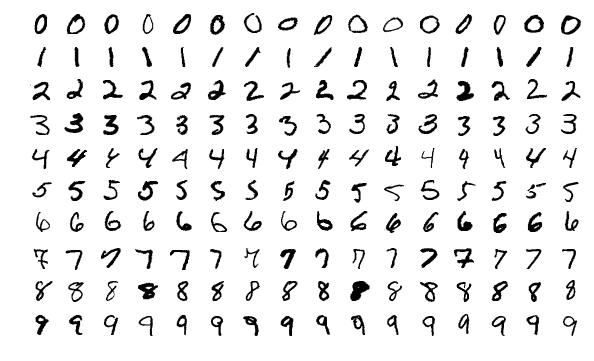
\includegraphics[width=0.75\textwidth]{content/section01/chapter01/figs/mnist.jpg}
    \caption{Sample images from the MNIST dataset.}
    \label{fig:mnist-samples}
\end{figure}

To begin, we import the essential PyTorch modules required for defining neural networks, optimization, dataset loading, and data transformation. The MNIST dataset is automatically downloaded in the original \texttt{.gz} compressed \texttt{ubyte} format. 

We apply a sequence of transformations: first converting each image to a PyTorch tensor, and then normalizing it using the dataset’s mean and standard deviation. The \texttt{DataLoader} wraps the dataset into iterable mini-batches and shuffles the training data at each epoch to improve learning.

\begin{tcolorbox}[codebox]
\begin{verbatim}
import torch
import torch.nn as nn
import torch.optim as optim

from torchvision import datasets, transforms
from torch.utils.data import DataLoader

transform = transforms.Compose([
    transforms.ToTensor(),
    transforms.Normalize((0.1307,), (0.3081,))
])

train_dataset = datasets.MNIST(root='./data', train=True, download=True, \
    transform=transform)

train_loader = DataLoader(train_dataset, batch_size=64, shuffle=True)

test_dataset = datasets.MNIST(root='./data', train=False, download=True, \
    transform=transform)

test_loader = DataLoader(test_dataset, batch_size=1000, shuffle=False)
\end{verbatim}
\end{tcolorbox}

We define a feedforward neural network by creating a subclass of \texttt{nn.Module}, which is the base class for all neural networks in PyTorch. The network structure is specified in two parts. 
\begin{itemize}
    \item The \texttt{\_\_init\_\_} method initializes the layers of the network. Here, the input layer is a fully connected linear layer that maps the \(28 \times 28 = 784\) input pixels to 128 hidden units. This is followed by a second hidden layer with 64 units, and finally an output layer with 10 units, corresponding to the ten digit classes (0 through 9).
    
    \item The \texttt{forward} method defines the forward pass computation. The input image is first flattened to a vector of size 784. Then it is passed sequentially through the linear layers and ReLU activation functions. Specifically, the ReLU activation is applied after the first and second linear transformations to introduce non-linearity, while the final output layer produces raw scores (logits) without an activation function, typically used with \texttt{CrossEntropyLoss}.
\end{itemize}

This architecture allows the model to learn a non-linear mapping from image pixels to digit class scores using two hidden layers.

\begin{tcolorbox}[codebox]
\begin{verbatim}
class FeedforwardNN(nn.Module):
    def __init__(self):
        super(FeedforwardNN, self).__init__()
        self.fc1 = nn.Linear(28*28, 128)
        self.relu = nn.ReLU()
        self.fc2 = nn.Linear(128, 64)
        self.fc3 = nn.Linear(64, 10)

    def forward(self, x):
        x = x.view(-1, 28*28)
        x = self.fc1(x)
        x = self.relu(x)
        x = self.fc2(x)
        x = self.relu(x)
        x = self.fc3(x)
        return x

model = FeedforwardNN()
\end{verbatim}
\end{tcolorbox}

Next, we define the loss function and optimizer. We use \texttt{CrossEntropyLoss}, which internally applies \texttt{LogSoftmax} followed by negative log-likelihood loss. For optimization, we use the Adam algorithm.

\begin{tcolorbox}[codebox]
\begin{verbatim}
criterion = nn.CrossEntropyLoss()
optimizer = optim.Adam(model.parameters(), lr=0.001)
\end{verbatim}
\end{tcolorbox}

We train the model for 5 epochs. In each iteration over the training data, we first set the model to training mode using \texttt{model.train()}. For each mini-batch, we clear the accumulated gradients from the previous step using \texttt{optimizer.zero\_grad()}, perform a forward pass to compute the predictions, and then compute the loss using the specified loss function. 

The backpropagation step is triggered by \texttt{loss.backward()}, which computes the gradients of the loss with respect to the model parameters. These gradients are then used by the optimizer to update the model parameters via \texttt{optimizer.step()}. A log of the loss is printed every 100 batches to monitor training progress.


\begin{tcolorbox}[codebox]
\begin{verbatim}
num_epochs = 5
for epoch in range(num_epochs):
    model.train()
    for batch_idx, (data, target) in enumerate(train_loader):
        optimizer.zero_grad()
        output = model(data)
        loss = criterion(output, target)
        loss.backward()
        optimizer.step()
        if batch_idx % 100 == 0:
            print(f"Epoch [{epoch+1}/{num_epochs}], \
                Batch [{batch_idx}/{len(train_loader)}], Loss: {loss.item():.4f}")
\end{verbatim}
\end{tcolorbox}


After training, we evaluate the model’s accuracy on the test set. We disable gradient computation and compare predicted labels with true labels to count the correct predictions.

\begin{tcolorbox}[codebox]
\begin{verbatim}
model.eval()
correct = 0
total = 0
with torch.no_grad():
    for data, target in test_loader:
        outputs = model(data)
        _, predicted = torch.max(outputs.data, 1)
        total += target.size(0)
        correct += (predicted == target).sum().item()

print(f'Test Accuracy of the model on 10,000 test images: \
    {100 * correct / total:.2f}%')
\end{verbatim}  
\end{tcolorbox}


The trained model achieves an accuracy of approximately \textbf{97.65\%} on the MNIST test dataset. 

This confirms that even a basic feedforward neural network, when trained appropriately using backpropagation, can effectively learn to classify digits from images.

\vspace{30pt}
\hrule

\chapter*{Review: Assignment 1}\cite{khapra2018deeplearning}
\addcontentsline{toc}{chapter}{Review: Assignment 1}

The objective of this assignment is to implement and use gradient descent (and its variants) with backpropagation for a classification task using a feedforward neural network. The task is to classify images from the Fashion-MNIST dataset (available on Kaggle) into one of 10 classes.

You are expected to implement the full network from scratch using Python. You may use \texttt{numpy} and \texttt{pandas}, but not any external deep learning libraries like PyTorch or TensorFlow. Use of the \texttt{argparse} module for command-line interface is mandatory. Set the seed to 1234 using \texttt{numpy.random.seed(1234)} to ensure replicability.

Your implementation must support the following command-line options.
\begin{verbatim}
--lr          : initial learning rate
--momentum    : momentum term (used only in momentum-based methods)
--num_hidden  : number of hidden layers
--sizes       : comma-separated list of sizes for each hidden layer
--activation  : activation function (tanh or sigmoid)
--loss        : loss function (sq for squared error, ce for cross entropy)
--opt         : optimization method (gd, momentum, nag, adam)
--batch_size  : batch size (1 or a multiple of 5)
--anneal      : halve learning rate if validation loss decreases (true/false)
--save_dir    : directory to save the model (weights and biases)
--expt_dir    : directory to save logs and predictions
--train       : path to training dataset
--test        : path to test dataset
\end{verbatim}

Your main script must be named \texttt{train.py} and should run using the following format.
\begin{verbatim}
python train.py --lr 0.01 --momentum 0.5 --num_hidden 3 --sizes 100,100,100 \
--activation sigmoid --loss sq --opt adam --batch_size 20 --anneal true \
--save_dir pa1/ --expt_dir pa1/exp1/ --train train.csv --test test.csv
\end{verbatim}

You must log your training and validation metrics every 100 steps in the files \texttt{log\_train.txt} and \texttt{log\_val.txt}, located in the \texttt{expt\_dir}. 

Each line must be formatted as follows.
\begin{verbatim}
Epoch 0, Step 100, Loss: <value>, Error: <value>, lr: <value>
\end{verbatim}
The error is the percentage of incorrect predictions (rounded to two decimal places).

You must also generate a file \texttt{predictions.csv} in the \texttt{expt\_dir}, containing the test set predictions with the following format.
\begin{verbatim}
id,label
0,3
1,2
2,8
...
9999,4
\end{verbatim}

Your report must be written in \LaTeX\ and include the following experimental plots.

\textbf{1. Varying hidden layer sizes} \\
For one, two, three, and four hidden layers, each with sizes in \{50, 100, 200, 300\}, plot the training and validation loss vs epoch (4 curves per plot, one for each size). Use sigmoid activation, cross entropy loss, Adam optimizer, batch size 20, and tune learning rate.

\textbf{2. Varying optimization algorithms} \\
Use 3 hidden layers of size 300 each and plot the training and validation loss using GD, momentum, NAG, and Adam.

\textbf{3. Activation functions comparison} \\
Compare sigmoid and tanh activations with 2 hidden layers of size 100, using Adam, cross entropy loss, and batch size 20.

\textbf{4. Loss functions comparison} \\
Compare squared error and cross entropy loss with 2 hidden layers of size 100, using sigmoid activation, Adam, and batch size 20.

\textbf{5. Batch size comparison} \\
Test with batch sizes 1, 20, 100, and 1000, using 2 hidden layers of size 100, sigmoid activation, cross entropy loss, and Adam.

Each plot must have epochs on the x-axis and loss on the y-axis, with clear legends.

You must create a file \texttt{supported.txt} listing the supported options for \texttt{--anneal}, \texttt{--opt}, \texttt{--loss}, and \texttt{--activation}, e.g.,
\begin{verbatim}
--anneal: true,false
--opt: gd,momentum,nag,adam
--loss: sq,ce
--activation: tanh,sigmoid
\end{verbatim}

All deliverables should be packaged into a single \texttt{tar.gz} archive named \texttt{RollNo\_backprop.tar.gz}, containing
\begin{verbatim}
- train.py
- run.sh (best performing command)
- any other Python scripts
- supported.txt
- report.pdf (written in LaTeX)
- predictions.csv
\end{verbatim}

Your task is to achieve an error rate below 8\% on the test set. Evaluation will be based on performance, code correctness, completeness, and the ability to support the specified hyperparameters. 

\qed

\afterpage{\blankpage}